\chapter{Fairness Verification with Feature Correlation}
	In this chapter, we discuss the extended experimental results as a continuation of Chapter~\ref{chapter:fvgm}.  


	\section{Extended Experimental Results}
	\label{fairness_fvgm_appendix:experiments}
	Each experiment is performed on Intel Xeon E$ 7-8857 $ v$2 $ CPUs with $ 16 $GB memory, $ 64 $bit Linux distribution based on Debian OS and clock speed $ 3 $ GHz.
	
	
	\begin{figure}
	\begin{center}
		\subfloat[]{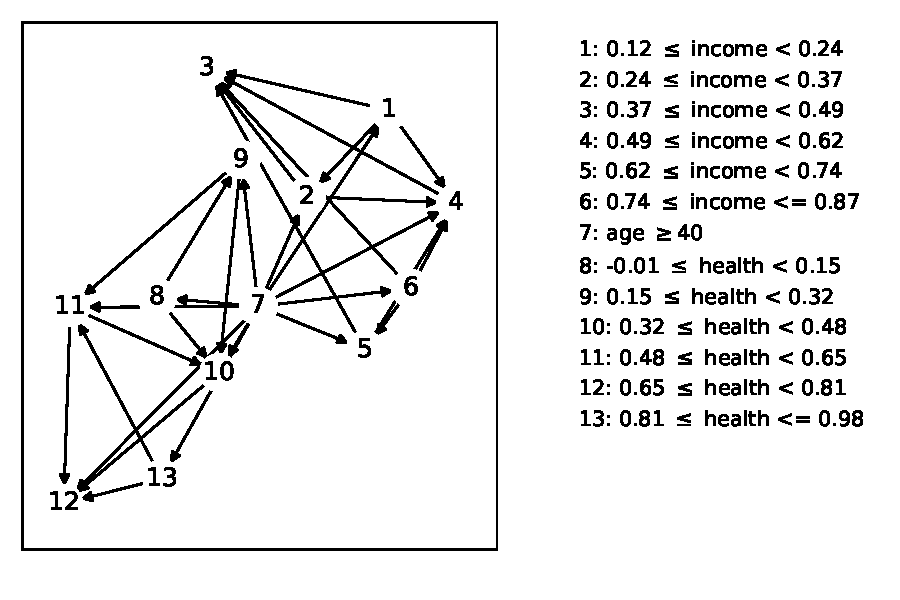
\includegraphics[scale=0.5]{figures/fairness/fvgm/synthetic_example_BN}\label{fairness_fvgm_fig:synthetic_bn}}
		
		\subfloat[]{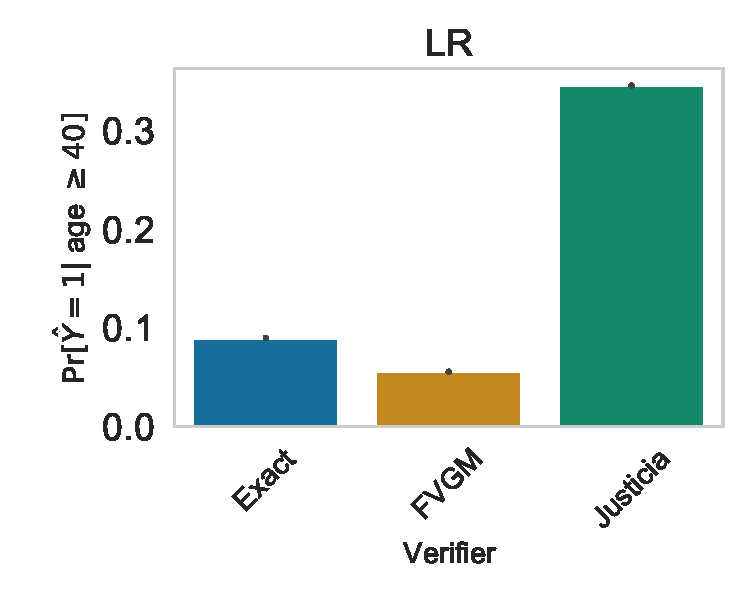
\includegraphics[scale=0.4]{figures/fairness/fvgm/sanity_ppv_max_PPV_LR}\label{fairness_fvgm_fig:synthetic_ppv_max_LR}}
		\subfloat[]{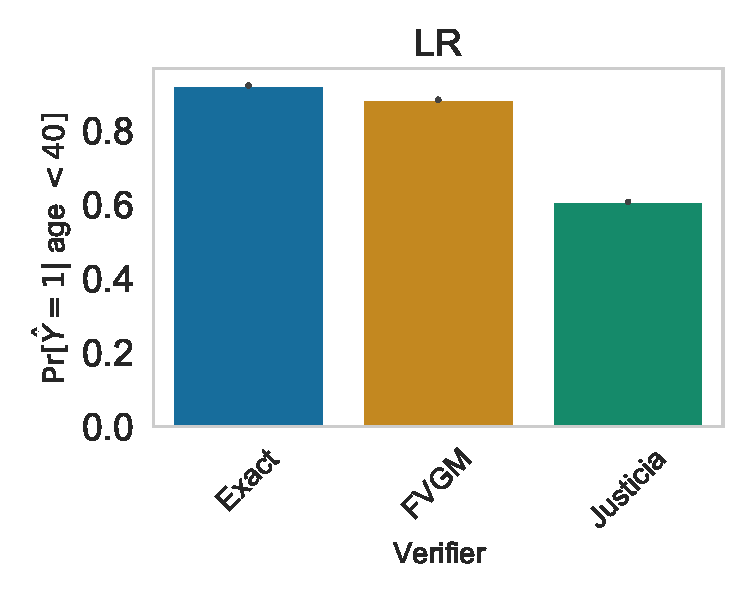
\includegraphics[scale=0.4]{figures/fairness/fvgm/sanity_ppv_min_PPV_LR}\label{fairness_fvgm_fig:synthetic_ppv_min_LR}}
		
		\subfloat[]{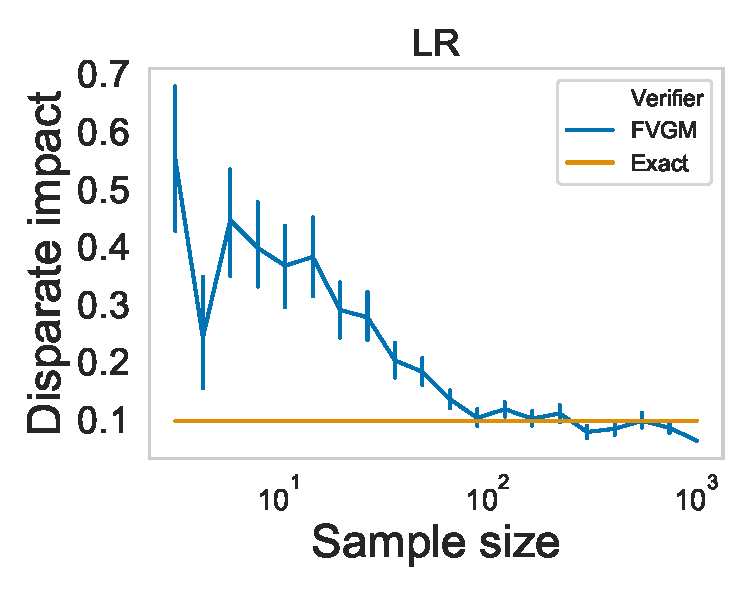
\includegraphics[scale=0.4]{figures/fairness/fvgm/sanity_sample_size_DI_LR}\label{fairness_fvgm_fig:synthetic_sample_size_LR_DI}}
		\subfloat[]{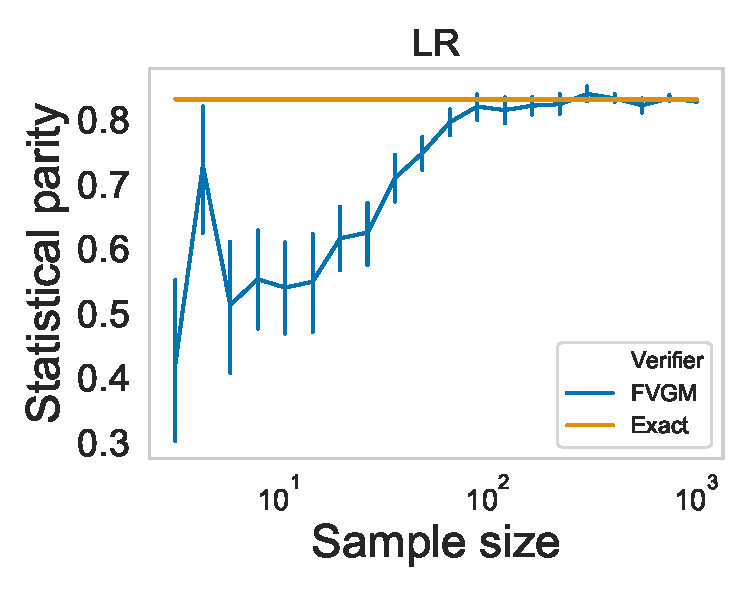
\includegraphics[scale=0.4]{figures/fairness/fvgm/sanity_sample_size_SPD_LR}\label{fairness_fvgm_fig:synthetic_sample_size_LR_SPD}}
	\end{center}
	
	\caption[Accuracy of {\fvgm} on logistic regression classifier]{
		Measuring accuracy of different fairness verifiers for Example~\ref{fairness_justicia_example:intro} on logistic regression classifier.}
	\label{fairness_fvgm_fig:synthetic_results}
\end{figure}


\begin{figure}
	\begin{center}
		\subfloat{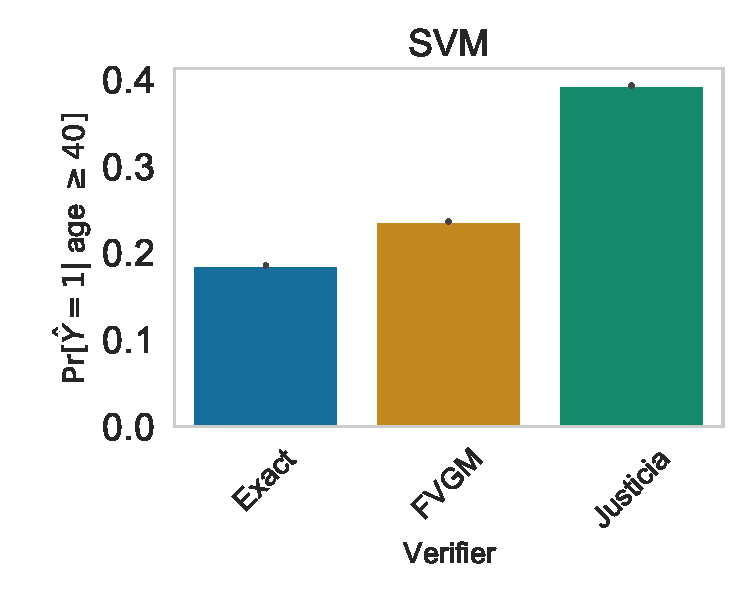
\includegraphics[scale=0.4]{figures/fairness/fvgm/sanity_ppv_max_PPV_SVM}}
		\subfloat{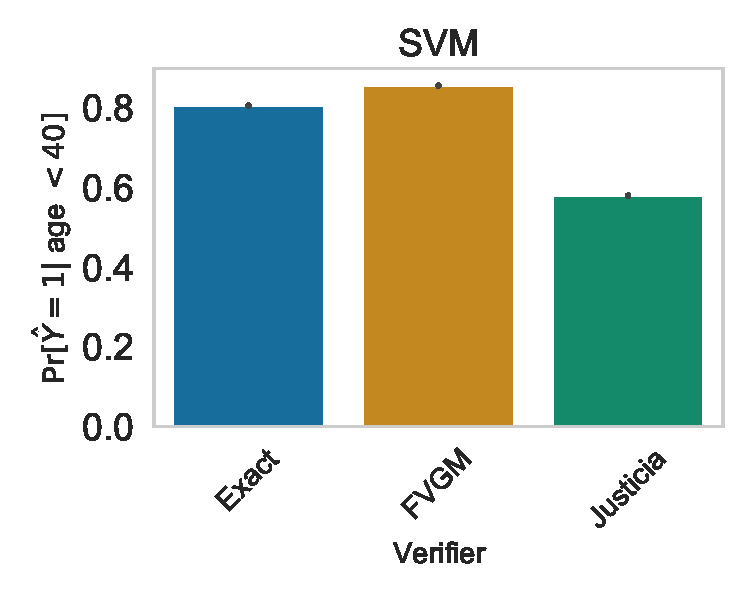
\includegraphics[scale=0.4]{figures/fairness/fvgm/sanity_ppv_min_PPV_SVM}}\\
		\subfloat{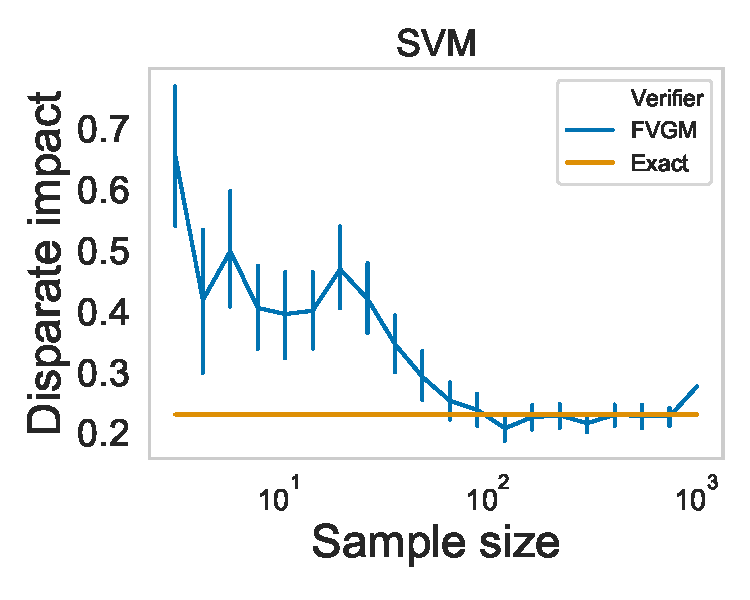
\includegraphics[scale=0.4]{figures/fairness/fvgm/sanity_sample_size_DI_SVM}}
		\subfloat{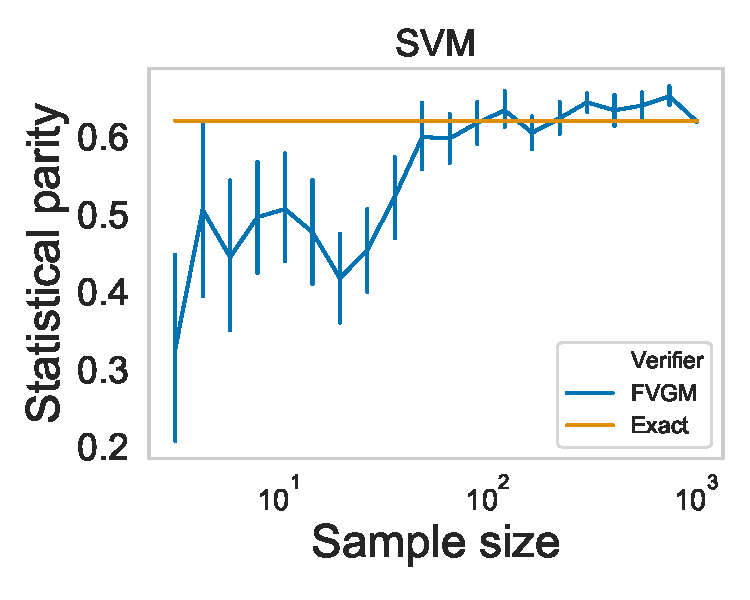
\includegraphics[scale=0.4]{figures/fairness/fvgm/sanity_sample_size_SPD_SVM}}
		
	\end{center}
	
	\caption[Accuracy of {\fvgm} on SVM classifier]{
		Measuring accuracy of different fairness verifiers for Example~\ref{fairness_justicia_example:intro} on SVM classifier.}
	\label{fairness_fvgm_fig:synthetic_results_SVM}
\end{figure}



	
	
	

		

	\subsection{Accuracy Comparison Among Different Verifiers}
	We have considered a synthetic problem for comparing accuracy among different verifiers. For Example~\ref{fairness_justicia_example:intro}, we consider `age $ \ge 40 $' as a Bernoulli random  variable with probability $ 0.5 $. For `income' feature ($ I $), we consider two Gaussian distributions $ \Pr[I | \text{age} \ge 40] \sim \mathcal{N}(0.6, 0.1) $ and $ \Pr[I | \text{age} < 40] \sim \mathcal{N}(0.4, 0.1) $ separated by two age groups. Moreover, for `fitness' feature ($ F $), we consider two Gaussian distributions $ \Pr[F | \text{age} \ge 40] \sim \mathcal{N}(0.7, 0.1) $ and $ \Pr[F | \text{age} < 40] \sim \mathcal{N}(0.3, 0.1) $. On this data, the trained LR and SVM classifier has decision boundary as $ 7.26I + 7.4F - 1.34A \ge 6.62 $ and $ 9.37I + 9.75F - 0.34A \ge 9.4 $, respectively.
	
	
	In Figure~\ref{fairness_fvgm_fig:synthetic_bn} we show the Bayesian Network on discretized features, in particular for income and fitness features. In Figure~\ref{fairness_fvgm_fig:synthetic_ppv_max_LR} and Figure~\ref{fairness_fvgm_fig:synthetic_ppv_min_LR}, we show PPVs of logistic regression classifier computed by different verifiers, where  {\fvgm} outputs closest to exactly computed values, in comparison with Justicia. In Figure~\ref{fairness_fvgm_fig:synthetic_sample_size_LR_DI} and Figure~\ref{fairness_fvgm_fig:synthetic_sample_size_LR_SPD}, we show the effect of sample size on {\fvgm} in measuring fairness metrics: disparate impact and statistical parity, where with increasing sample size, the estimate becomes more accurate. Similar observations are recorded for SVM classifier in Figure~\ref{fairness_fvgm_fig:synthetic_results_SVM}.
	

		\begin{figure}
		\begin{center}
			\subfloat{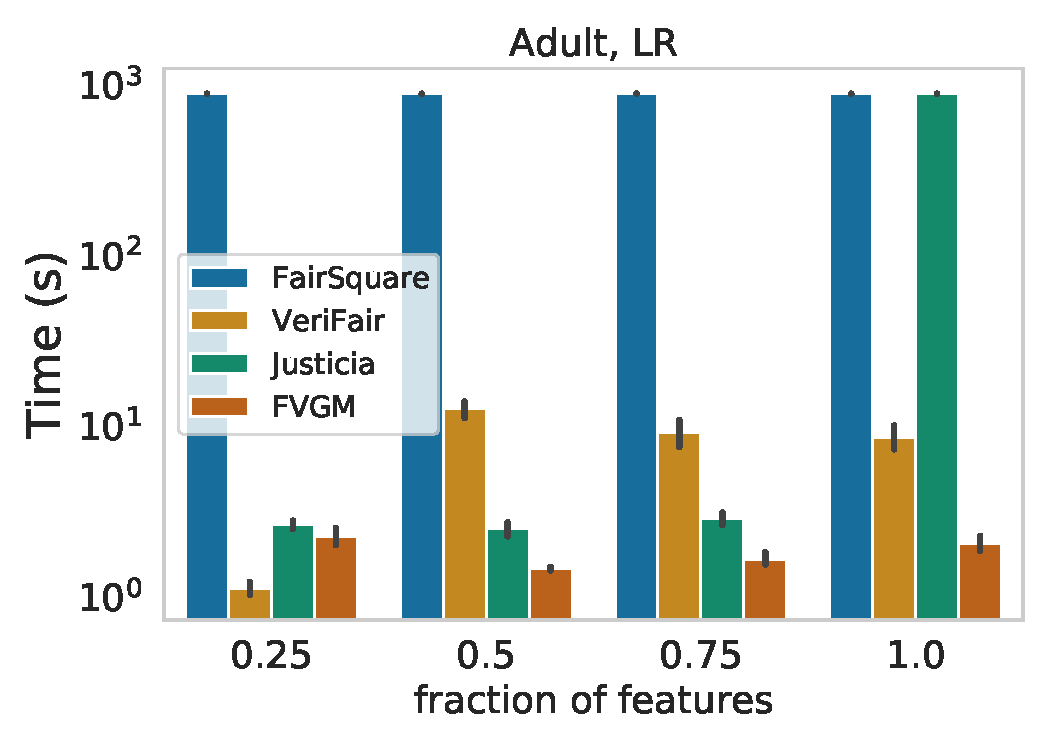
\includegraphics[scale=0.4]{figures/fairness/fvgm/time_vary_features_Adult_LR}}
			\subfloat{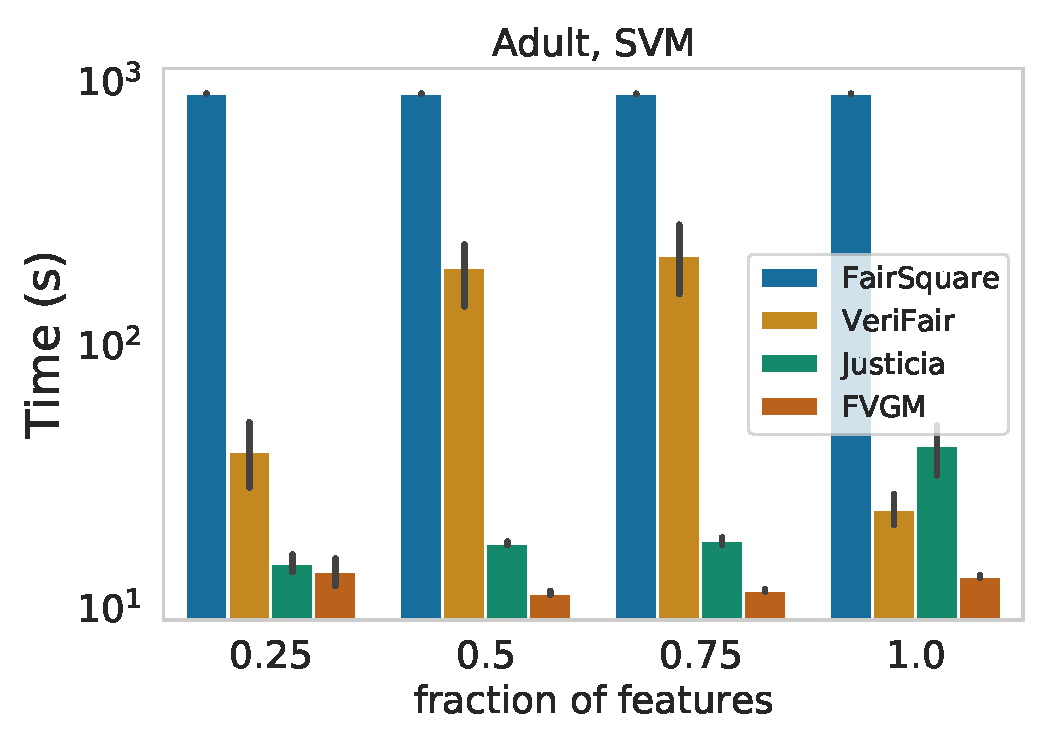
\includegraphics[scale=0.4]{figures/fairness/fvgm/time_vary_features_Adult_SVM}}	\\		
			\subfloat{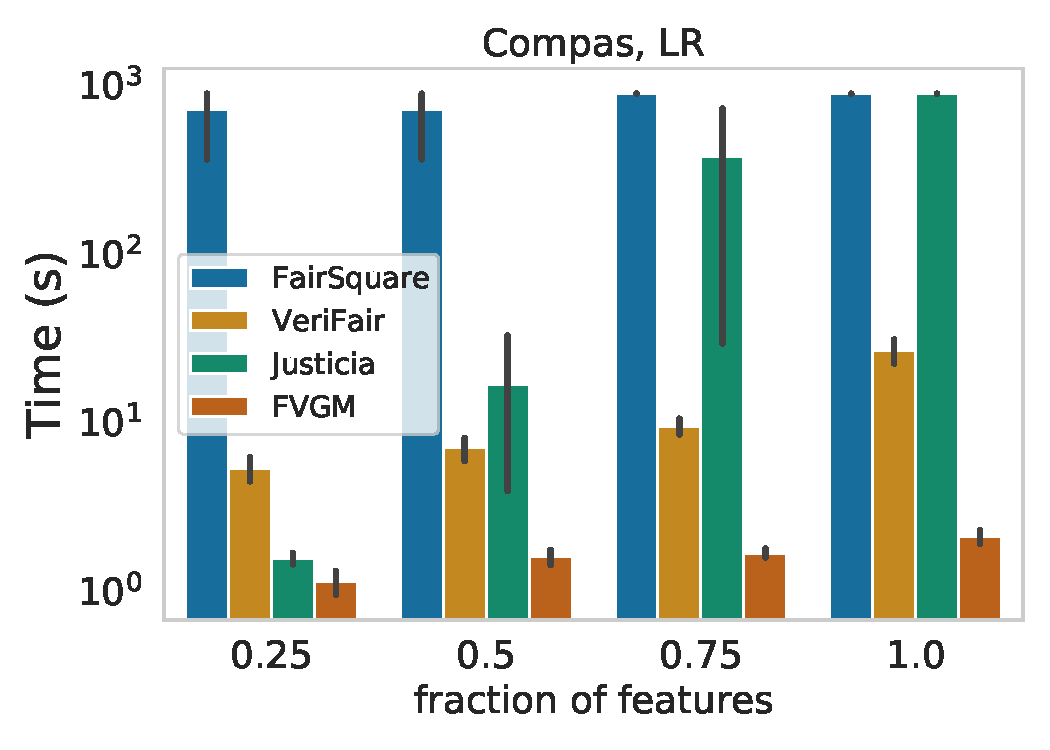
\includegraphics[scale=0.4]{figures/fairness/fvgm/time_vary_features_Compas_LR}}
			\subfloat{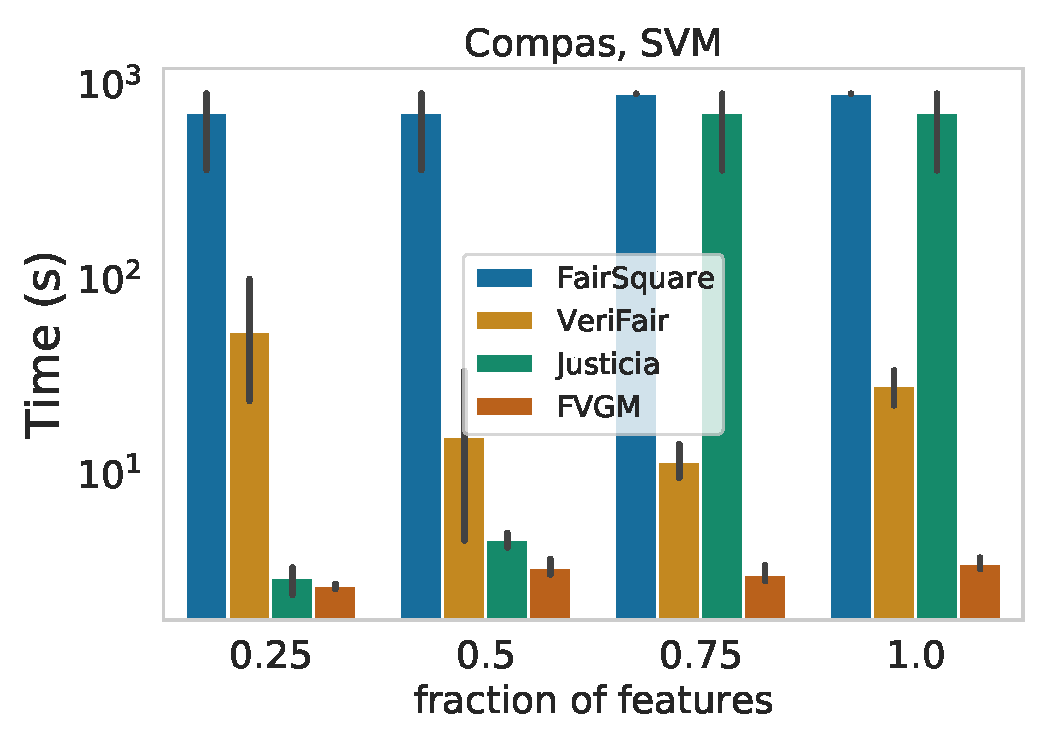
\includegraphics[scale=0.4]{figures/fairness/fvgm/time_vary_features_Compas_SVM}}\\
			
			\subfloat{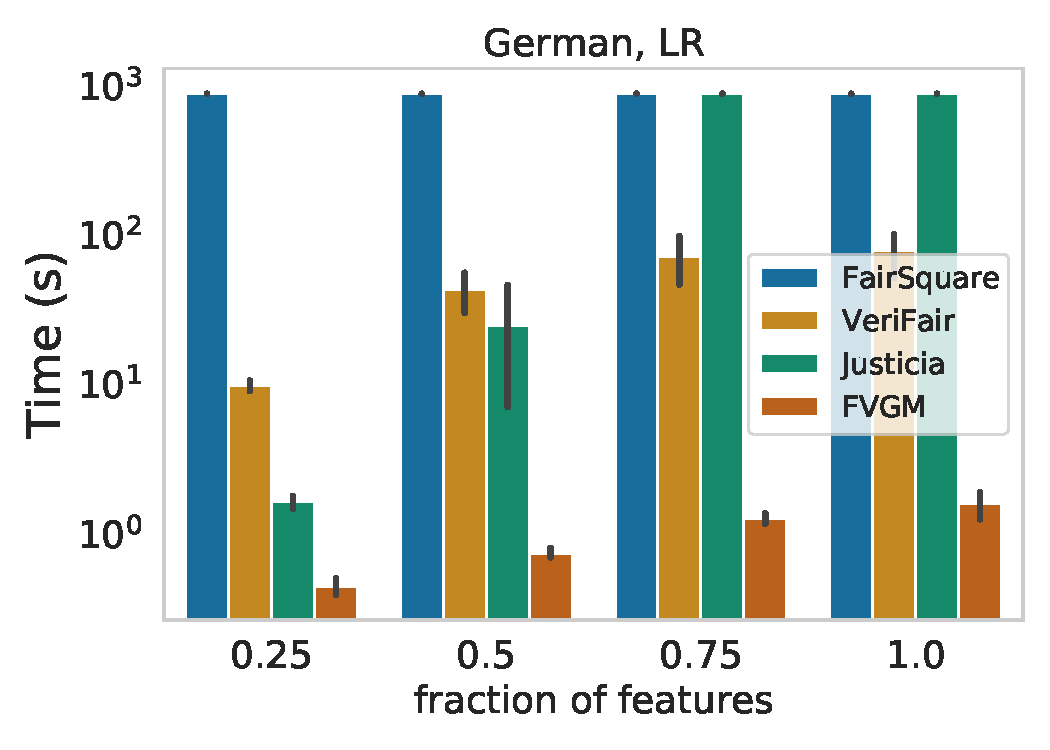
\includegraphics[scale=0.4]{figures/fairness/fvgm/time_vary_features_German_LR}}
			\subfloat{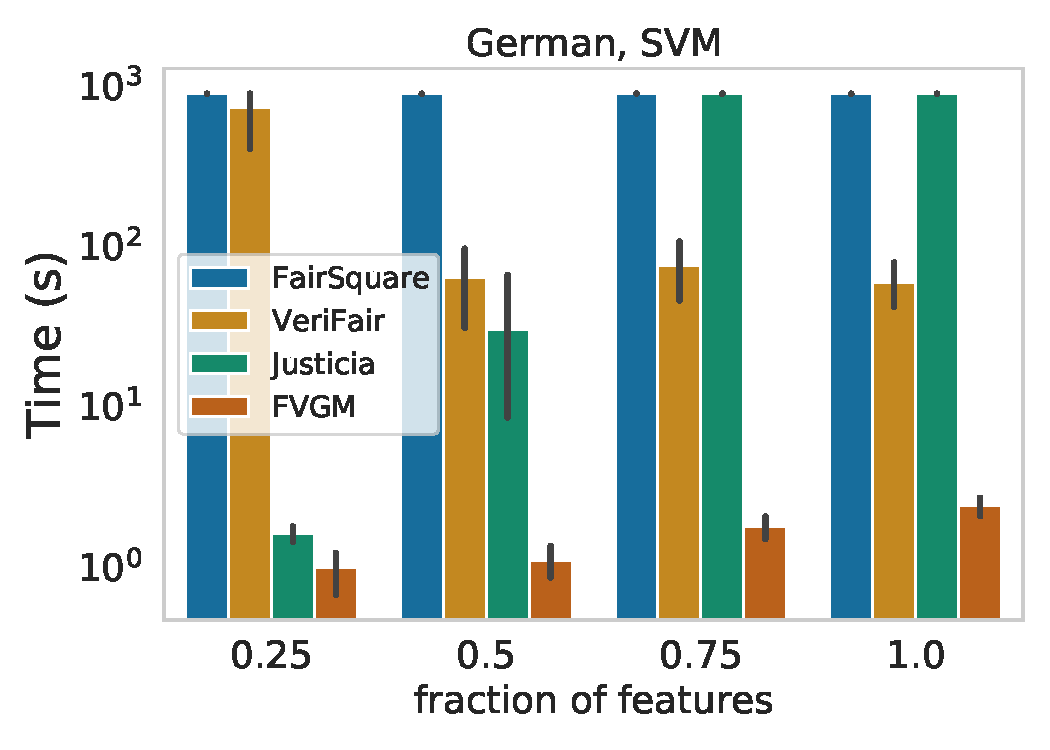
\includegraphics[scale=0.4]{figures/fairness/fvgm/time_vary_features_German_SVM}}		\\
			\subfloat{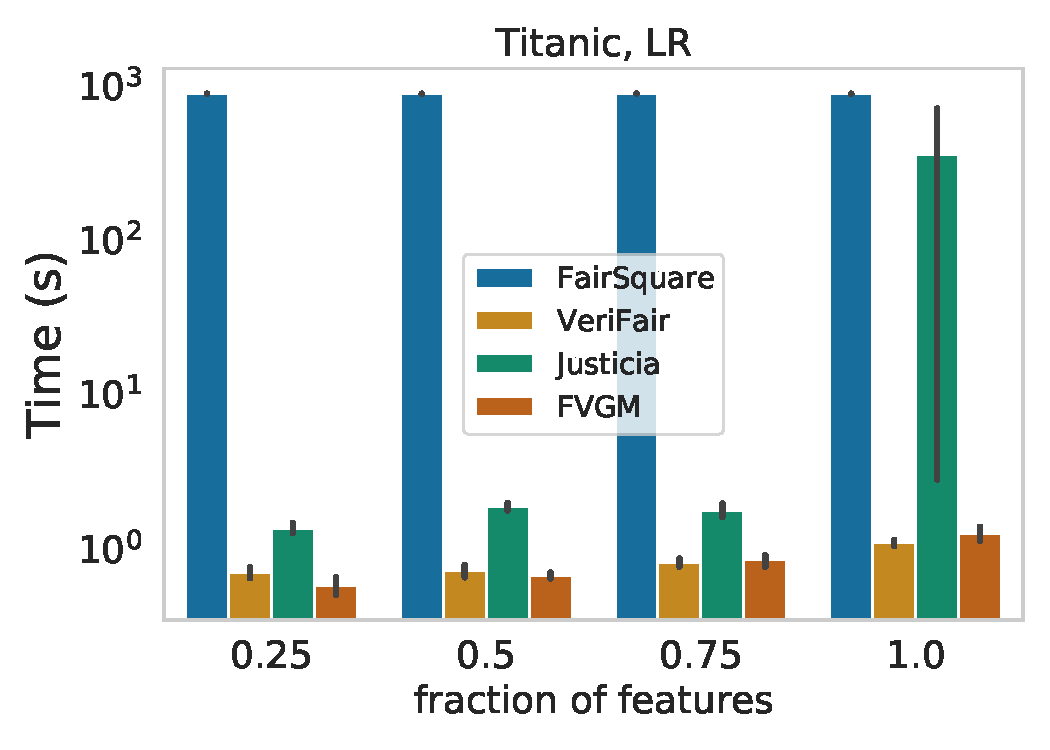
\includegraphics[scale=0.4]{figures/fairness/fvgm/time_vary_features_Titanic_LR}}
			\subfloat{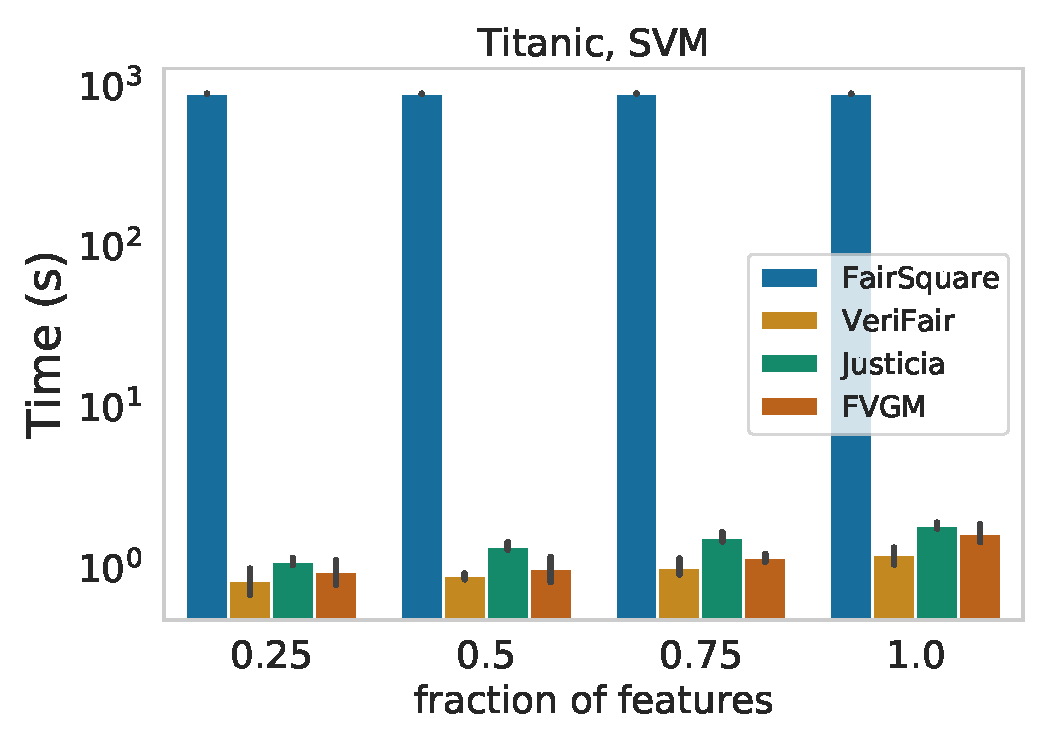
\includegraphics[scale=0.4]{figures/fairness/fvgm/time_vary_features_Titanic_SVM}}\\
			
%			\subfloat{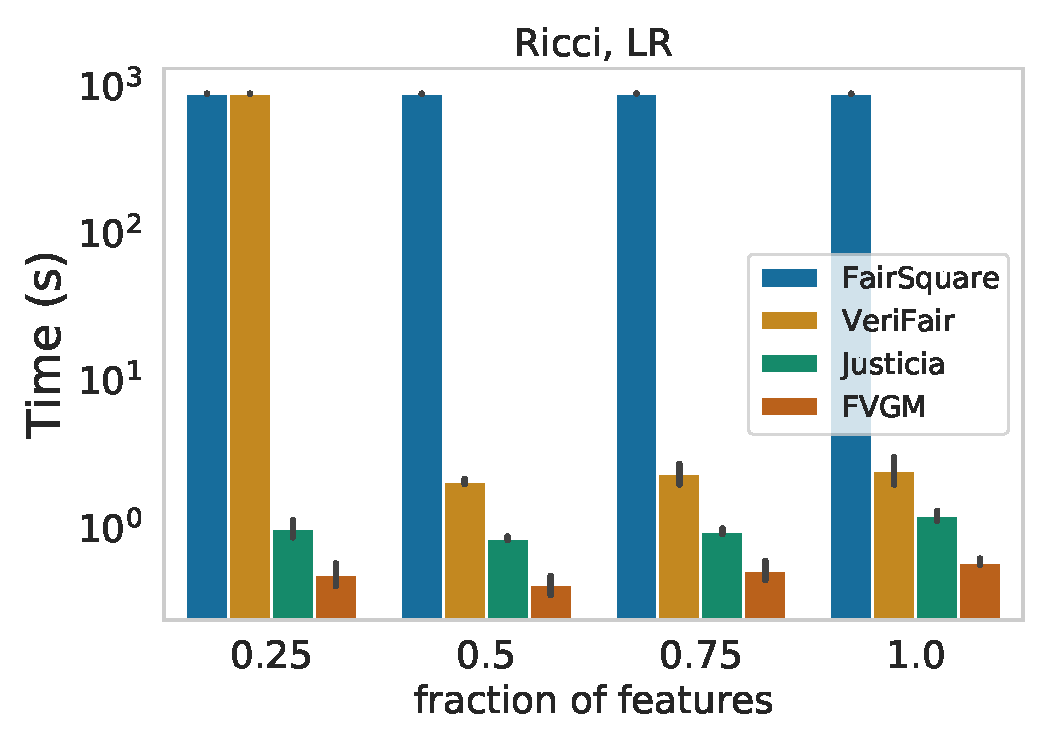
\includegraphics[scale=0.4]{figures/fairness/fvgm/time_vary_features_Ricci_LR}}
%			\subfloat{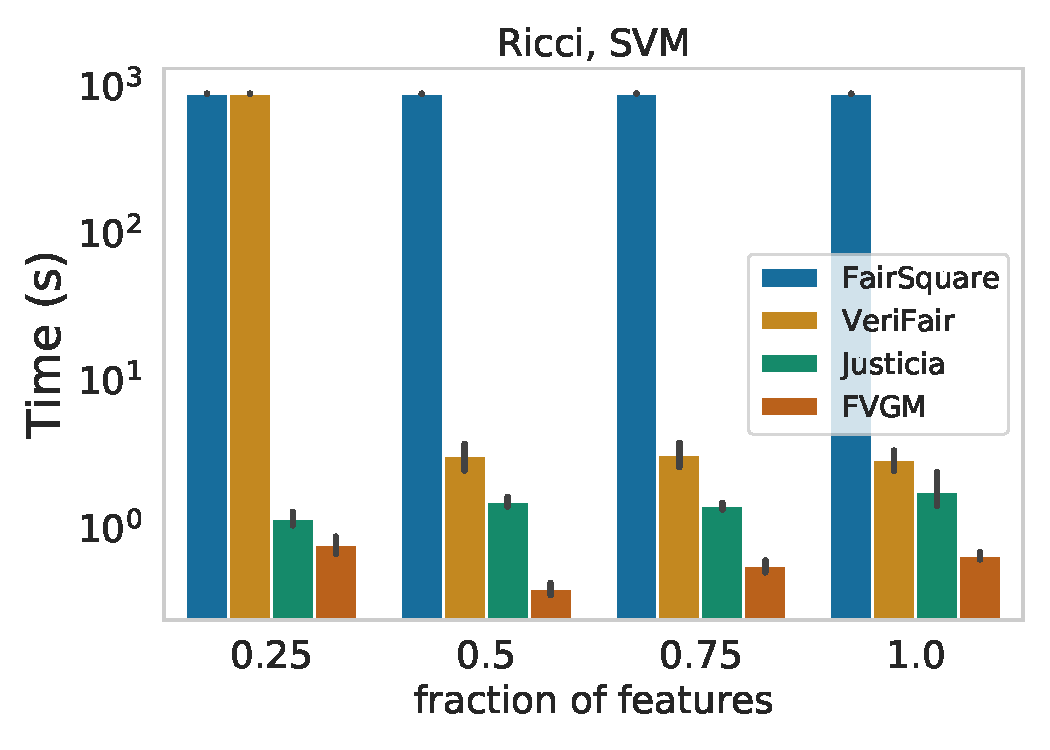
\includegraphics[scale=0.4]{figures/fairness/fvgm/time_vary_features_Ricci_SVM}}
%			
			\caption[Ablation study: effect of the number of features]{Effect of number of features on the runtime of different datasets for LR and SVM classifiers.}
			\label{fairness_fvgm_fig:time_vary_features}
			
			
			
		\end{center}
		
		
	\end{figure}
	
	
	\subsection{Scalability Comparison Among Different Verifiers}
	
	In Figure~\ref{fairness_fvgm_fig:time_vary_features}, we present the runtime of different fairness verifiers while varying the number of features in different datasets. We observe that with an increase of features, the runtime increases in general.
	
	
	
	
	
	
	
	
	\begin{figure}
	\begin{center}
		\subfloat{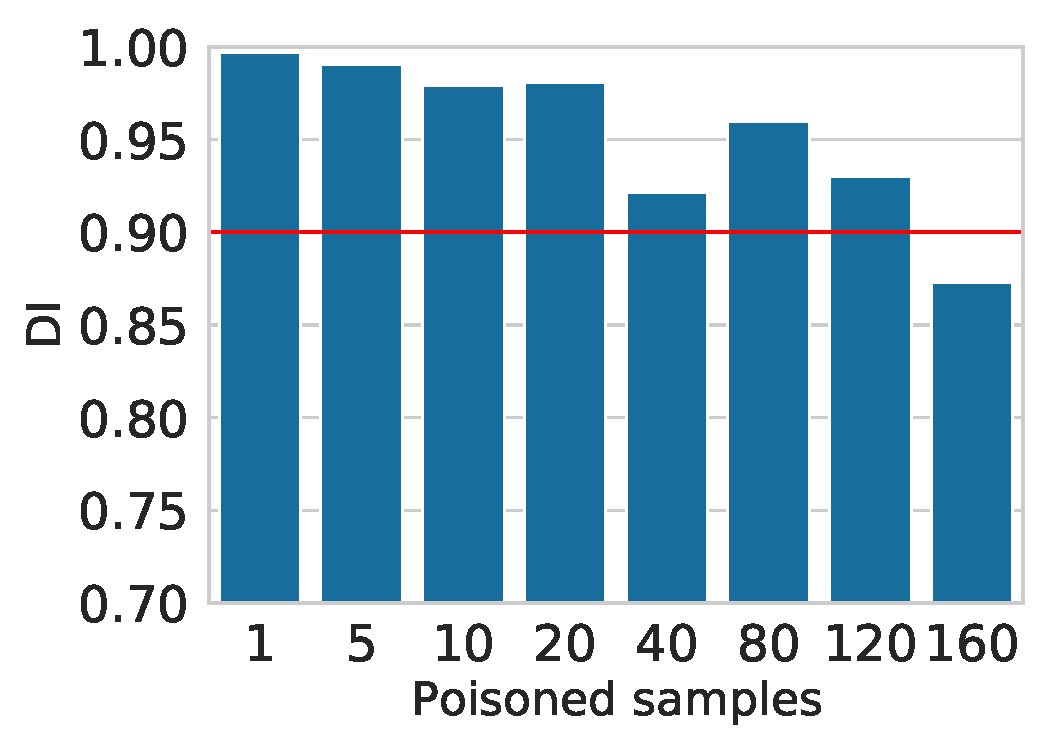
\includegraphics[scale=0.35]{figures/fairness/fvgm/disp_fairness_attack}}
		\subfloat{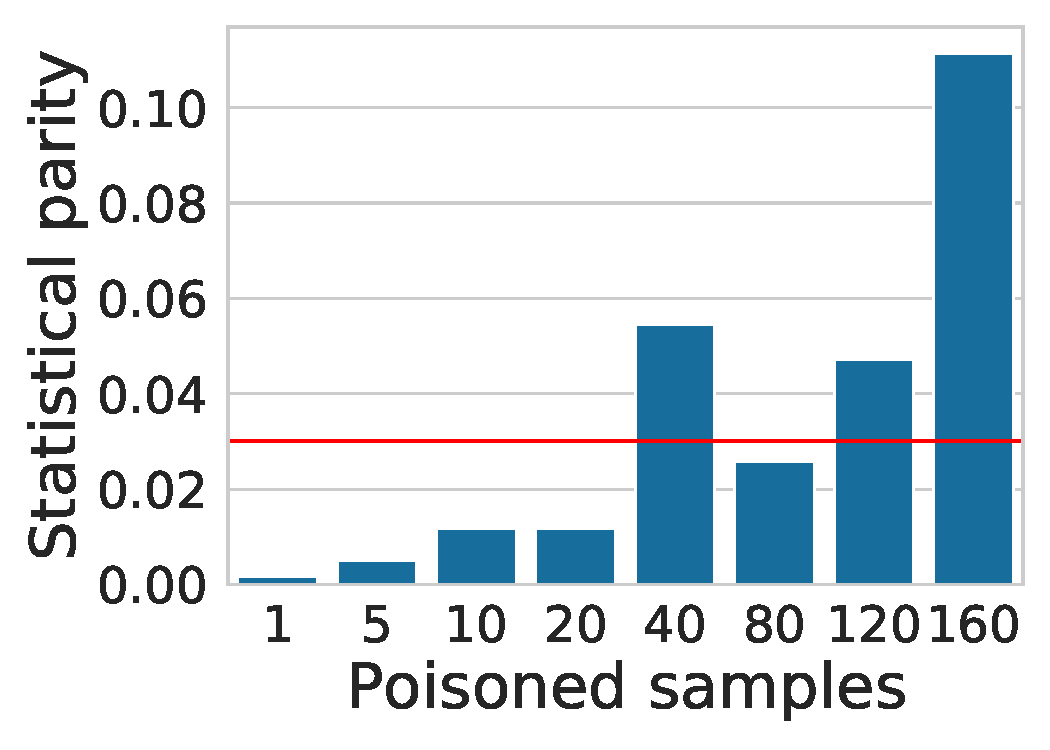
\includegraphics[scale=0.35]{figures/fairness/fvgm/stat_fairness_attack}}\\
	\end{center}
	\caption[Verifying fairness poisoning attack using {\fvgm}]{Verifying fairness poisoning attack using {\fvgm}. The red line denotes safety margin, which being exceeded denotes system-vulnerability by the attack algorithm. As the number of poisoned samples increase, disparate impact (DI) decreases and statistical parity (SP)  increases.}
	\label{fairness_fvgm_fig:attack_extended}
\end{figure}

	%\clearpage

\begin{table}[t!]
    \centering
        \setlength{\tabcolsep}{.3em}
%        \vspace*{-.3em}
            \begin{tabular}{lrrrrrrrrrrrrrrr}
                \toprule
                Dataset   & \multicolumn{3}{c}{Ricci} & \multicolumn{3}{c}{Titanic} & \multicolumn{3}{c}{COMPAS} &  \multicolumn{3}{c}{Adult} &
                \multicolumn{3}{c}{German} \\ 
                
                \cmidrule(lll){2-4}
                \cmidrule(lr){5-7}
                \cmidrule(lr){8-10}
                \cmidrule(lr){11-13}
                \cmidrule(lr){14-16}
                

                Classifier & 
                LR & SVC & DT &
                LR & SVC & DT &
                LR & SVC & DT &
                LR & SVC & DT &
                LR & SVC & DT \\
				 \midrule

{\framework} &  $ \textbf{0.1} $  &  $ \textbf{0.1} $  &  $ \textbf{0.1} $  &  $ \textbf{0.1} $  &  $ \textbf{0.1} $  &  $ 1.6 $  &  $ \textbf{0.4} $  &  $ \textbf{0.5} $  &  $ 121.7 $  &  $ \textbf{0.9} $  &  $ 1.8 $  &  $ \textbf{0.3} $  &  $ \textbf{1.4} $  &  $ \textbf{1.4} $  &  $ 2.3 $  \\ 
Justicia &  $ 2.2 $  &  $ 2.2 $  &  $ \textbf{0.1} $  &  $ 0.3 $  &  $ 0.2 $  &  $ \textbf{0.3} $  & \textemdash & \textemdash &  $ \textbf{0.3} $  & \textemdash &  $ \textbf{1.7} $  &  $ 0.4 $  & \textemdash & \textemdash &  $ \textbf{0.2} $  \\ 
VeriFair &  $ 2.0 $  &  $ 1.8 $  &  $ 1.9 $  &  $ 0.5 $  &  $ 0.4 $  &  $ 17.2 $  &  $ 12.2 $  &  $ 11.6 $  &  $ 377.1 $  &  $ 7.3 $  &  $ 21.7 $  &  $ 57.9 $  &  $ 19.2 $  &  $ 28.8 $  &  $ 78.5 $  \\ 
FairSquare & \textemdash & \textemdash &  $ 4.6 $  & \textemdash & \textemdash &  $ 432.9 $  & \textemdash & \textemdash & \textemdash & \textemdash & \textemdash & \textemdash & \textemdash & \textemdash & \textemdash \\ 



















	
		
			
				
				
				
				
				
				
				


    \end{tabular}
\caption{Scalability of different verifiers in terms of execution time (in seconds).  DT and LR refer to decision tree and logistic regression respectively. `\textemdash'~ refers to timeout. \red{Restricted experiments with Boolean single sensitive attribute.}}
\label{tab:FS_VF_Justicia}
%\vspace*{-1em}
\end{table}








\begin{table}[t!]
	\centering
	\setlength{\tabcolsep}{.3em}
	%        \vspace*{-.3em}
	\begin{tabular}{lrrrrrrrrrrrrrrr}
		\toprule
		Dataset   & \multicolumn{3}{c}{Ricci} & \multicolumn{3}{c}{Titanic} & \multicolumn{3}{c}{COMPAS} &  \multicolumn{3}{c}{Adult} &
		\multicolumn{3}{c}{German} \\ 
		
		\cmidrule(lr){2-4}
		\cmidrule(lr){5-7}
		\cmidrule(lr){8-10}
		\cmidrule(lr){11-13}
		
		
		Classifier & 
		LR & SVC & DT &
		LR & SVC & DT &
		LR & SVC & DT &
		LR & SVC & DT &
		LR & SVC & DT \\
		\midrule
		
		{\framework} &  $ 0.86 $  &  $ 1.0 $  &  $ 1.0 $  &  $ 0.16 $  &  $ 0.0 $  &  $ 0.59 $  &  $ 0.74 $  &  $ 0.85 $  &  $ 0.94 $  &  $ 0.65 $  &  $ 1.0 $  &  $ 0.49 $  &  $ 0.82 $  &  $ 0.9 $  &  $ 0.94 $  \\ 
		Justicia &  $ 0.26 $  &  $ 0.36 $  &  $ 0.3 $  &  $ 0.14 $  &  $ 0.0 $  &  $ 0.55 $  & \textemdash & \textemdash &  $ 0.79 $  & \textemdash &  $ 0.85 $  &  $ 0.22 $  & \textemdash & \textemdash &  $ 0.89 $  \\ 
		VeriFair &  $ 0.28 $  &  $ 0.4 $  &  $ 0.49 $  &  $ 0.1 $  &  $ 0.0 $  &  $ 0.87 $  &  $ 0.79 $  &  $ 0.74 $  &  $ 0.97 $  &  $ 0.79 $  &  $ 0.88 $  &  $ 0.93 $  &  $ 0.66 $  &  $ 0.64 $  &  $ 0.89 $  \\ 
		FairSquare & \textemdash & \textemdash &  $ 0.52 $  & \textemdash & \textemdash &  $ 0.87 $  & \textemdash & \textemdash & \textemdash & \textemdash & \textemdash & \textemdash & \textemdash & \textemdash & \textemdash \\ 
		
		
		
		
		
		
		
		
		
		
		
		
		
		
		
	\end{tabular}
	\caption{Computed disparate impact by different fairness verifiers on different datasets and classifiers.  DT and LR refer to decision tree and logistic regression respectively. `\textemdash'~ refers to timeout.}
	\label{tab:FS_VF_Justicia}
	%\vspace*{-1em}
\end{table}
	%
\begin{figure}
		\begin{center}
			\subfloat[]{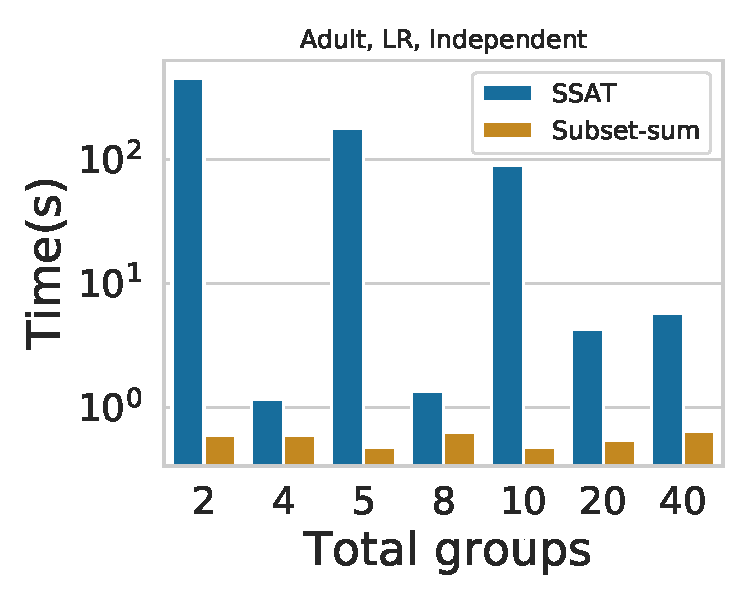
\includegraphics[scale=0.25]{figures/ssat_vs_subsetsum_Independent_Adult_LR}}
			\subfloat[]{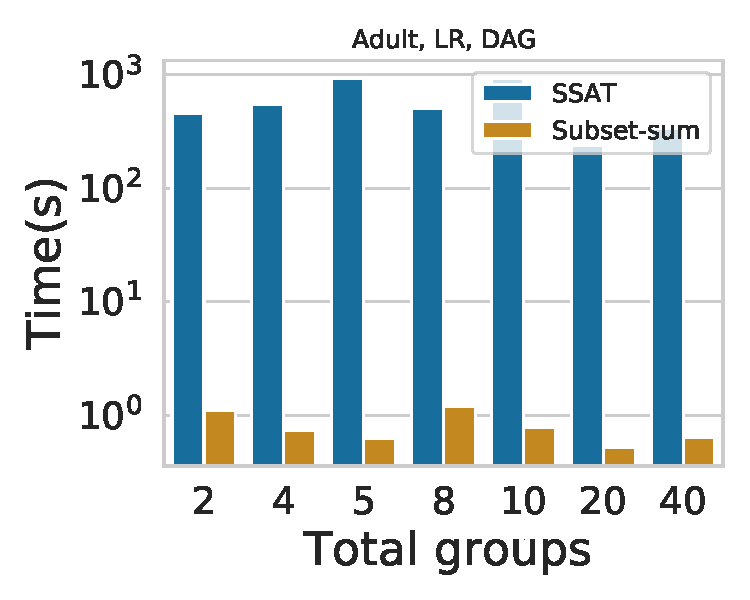
\includegraphics[scale=0.25]{figures/ssat_vs_subsetsum_DAG_Adult_LR}}
			\subfloat[]{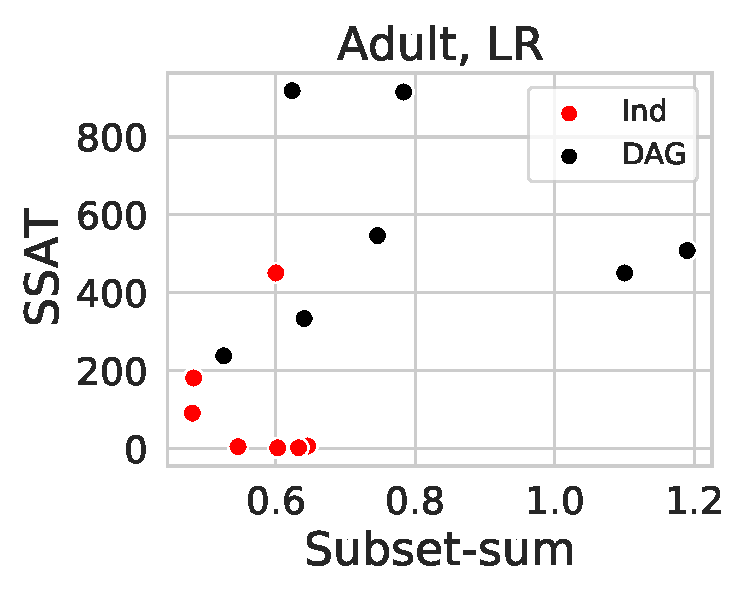
\includegraphics[scale=0.25]{figures/ssat_vs_subsetsum_time_scatter_plot_Adult_LR}}\\
			
			\subfloat[]{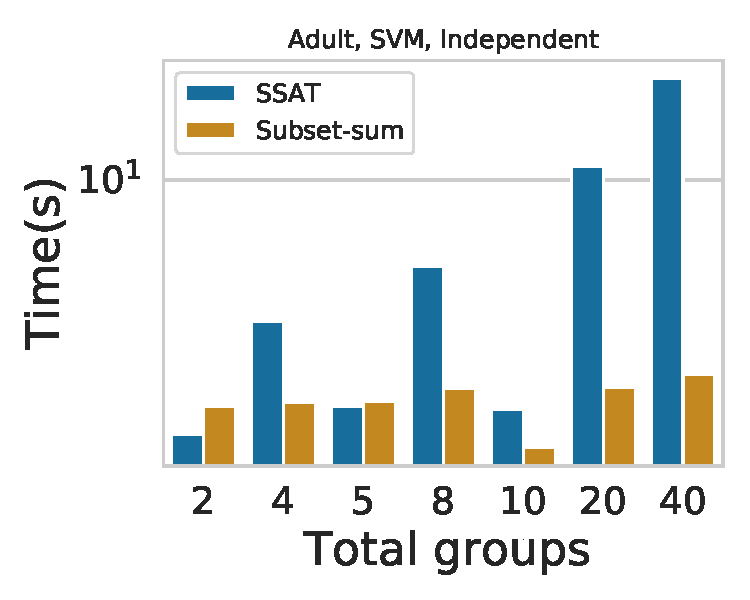
\includegraphics[scale=0.25]{figures/ssat_vs_subsetsum_Independent_Adult_SVM}}
			\subfloat[]{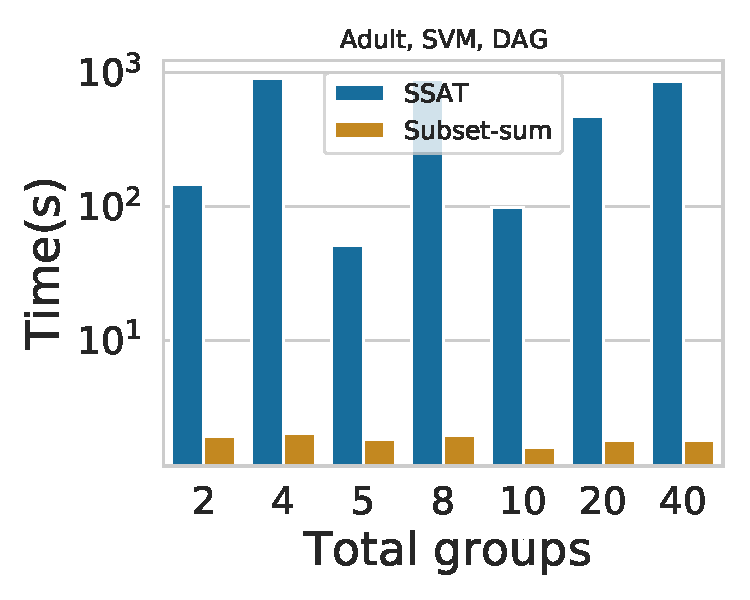
\includegraphics[scale=0.25]{figures/ssat_vs_subsetsum_DAG_Adult_SVM}}
			\subfloat[]{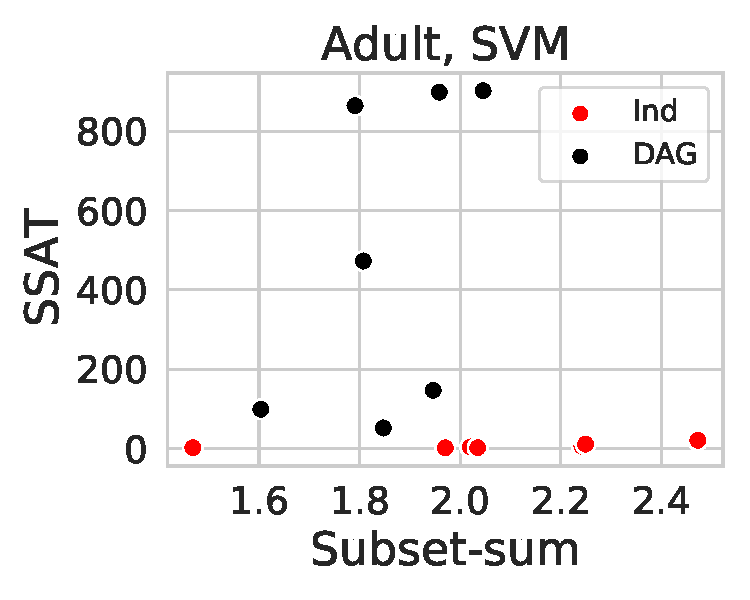
\includegraphics[scale=0.25]{figures/ssat_vs_subsetsum_time_scatter_plot_Adult_SVM}}\\
			
			
			\subfloat[]{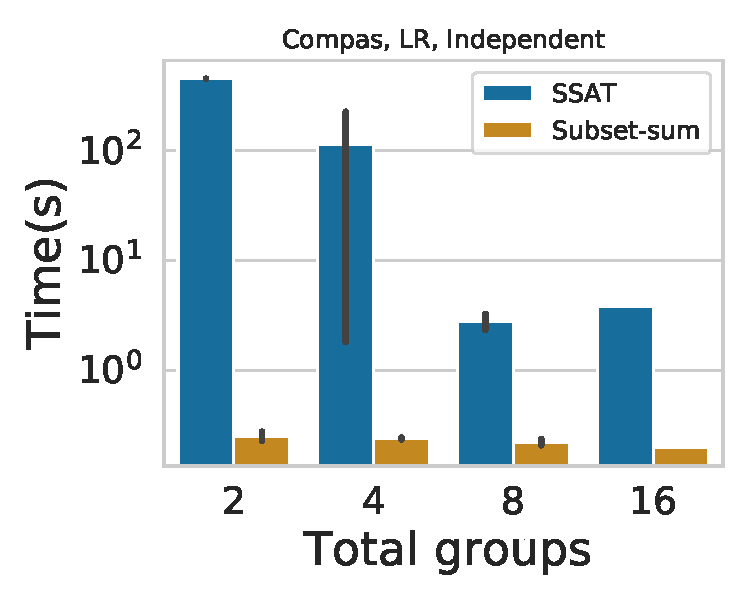
\includegraphics[scale=0.25]{figures/ssat_vs_subsetsum_Independent_Compas_LR}}
			\subfloat[]{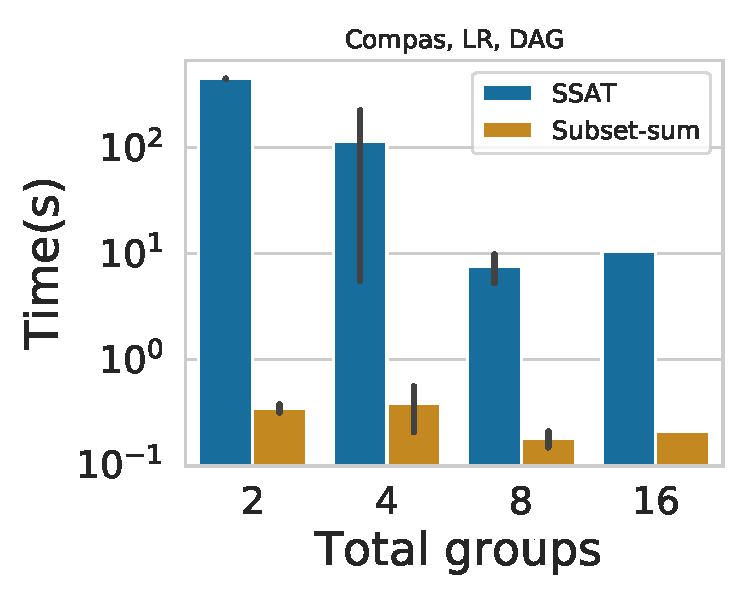
\includegraphics[scale=0.25]{figures/ssat_vs_subsetsum_DAG_Compas_LR}}
			\subfloat[]{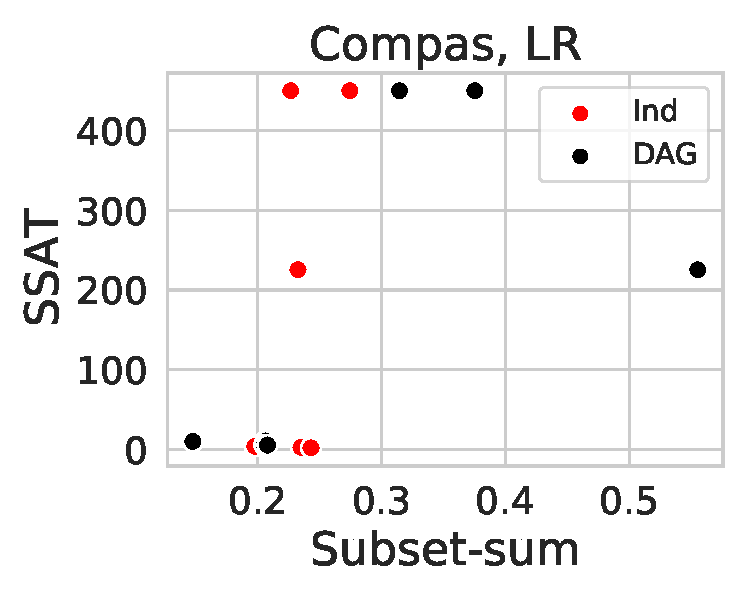
\includegraphics[scale=0.25]{figures/ssat_vs_subsetsum_time_scatter_plot_Compas_LR}}\\
			
			\subfloat[]{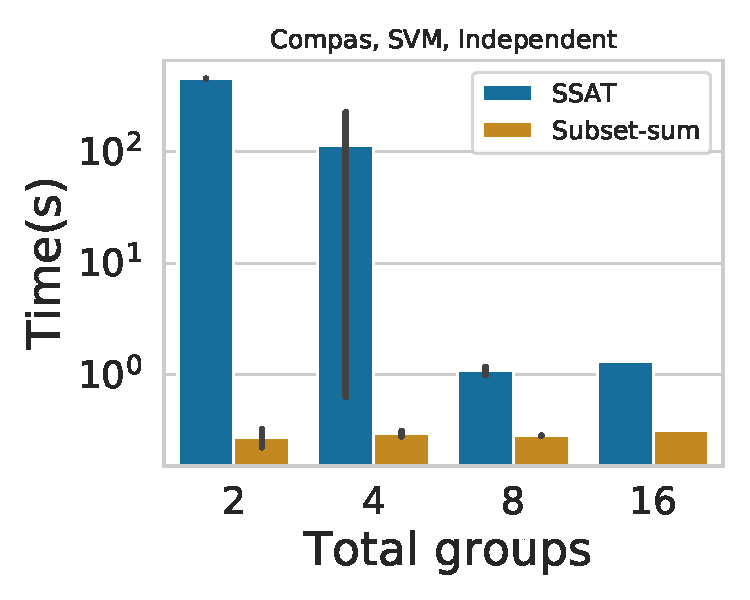
\includegraphics[scale=0.25]{figures/ssat_vs_subsetsum_Independent_Compas_SVM}}
			\subfloat[]{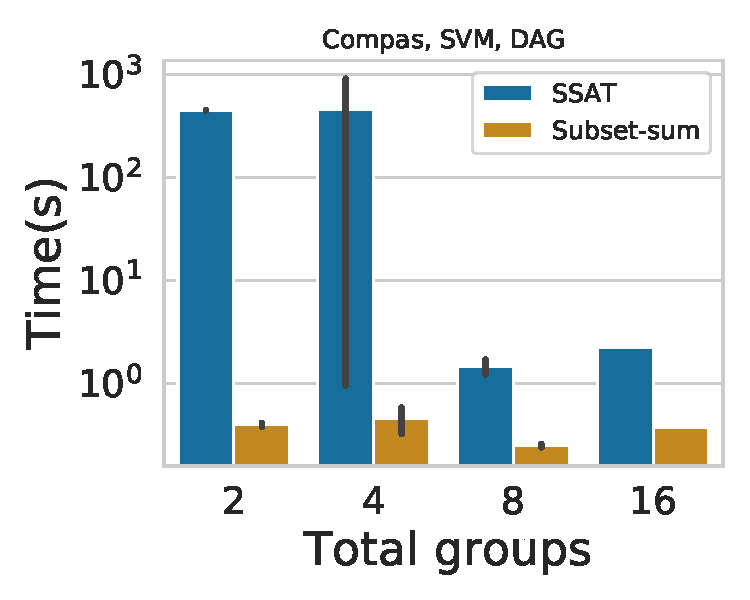
\includegraphics[scale=0.25]{figures/ssat_vs_subsetsum_DAG_Compas_SVM}}
			\subfloat[]{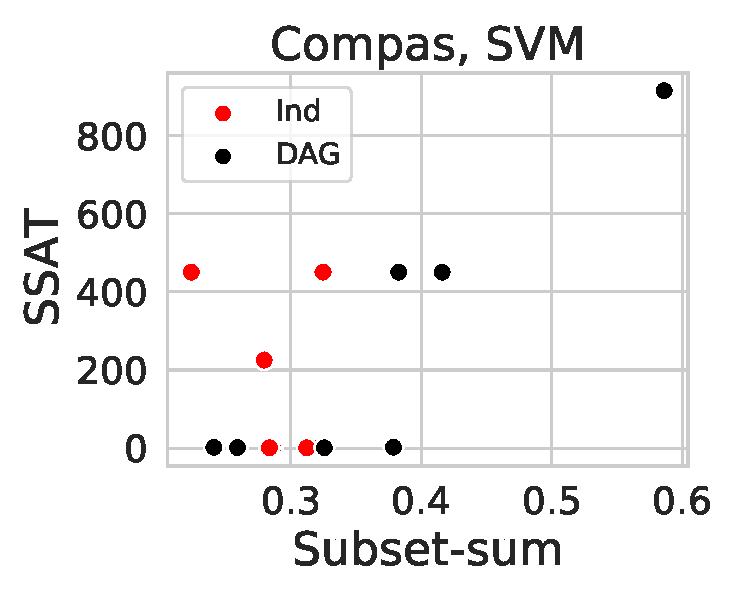
\includegraphics[scale=0.25]{figures/ssat_vs_subsetsum_time_scatter_plot_Compas_SVM}}\\
			
			\subfloat[]{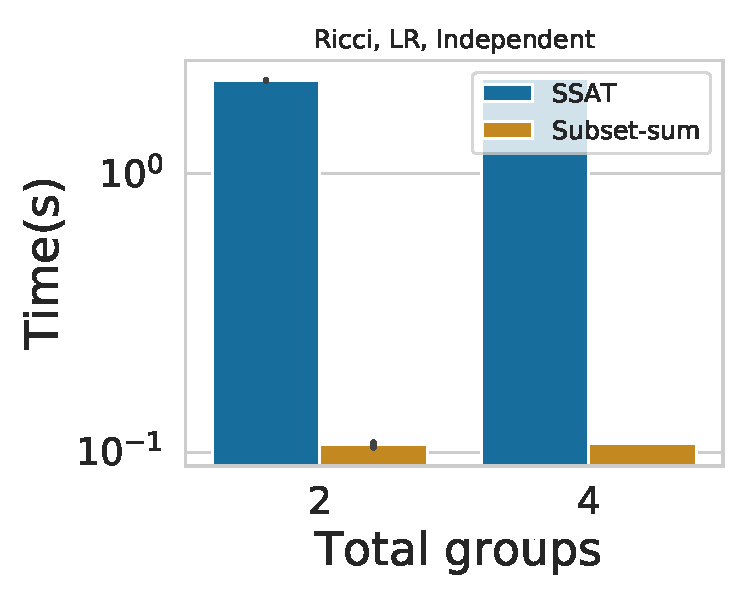
\includegraphics[scale=0.25]{figures/ssat_vs_subsetsum_Independent_Ricci_LR}}
			\subfloat[]{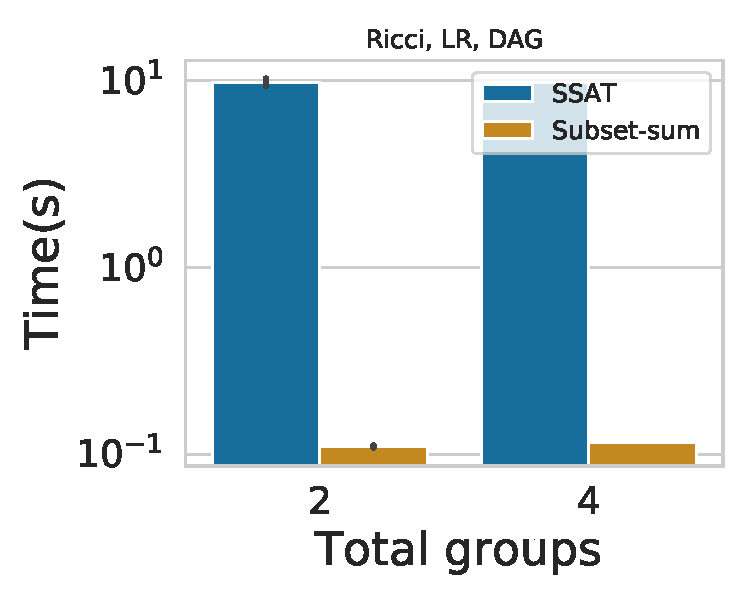
\includegraphics[scale=0.25]{figures/ssat_vs_subsetsum_DAG_Ricci_LR}}
			\subfloat[]{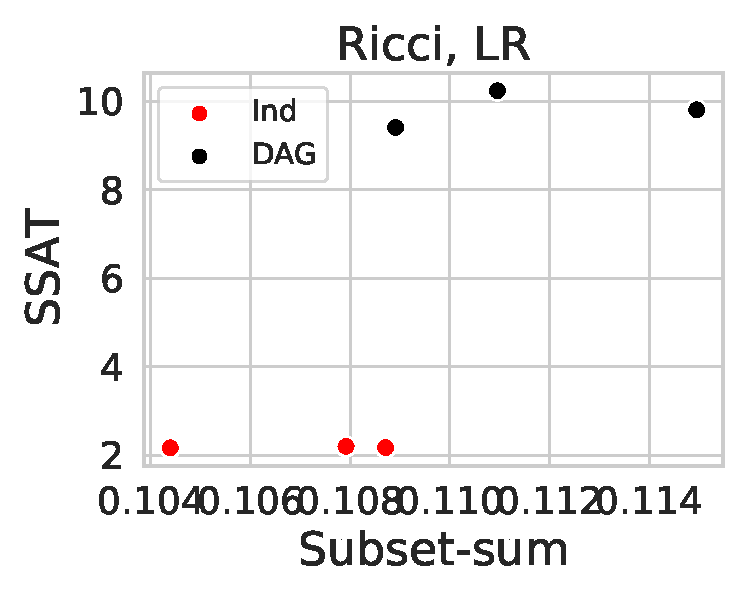
\includegraphics[scale=0.25]{figures/ssat_vs_subsetsum_time_scatter_plot_Ricci_LR}}\\
			
			\subfloat[]{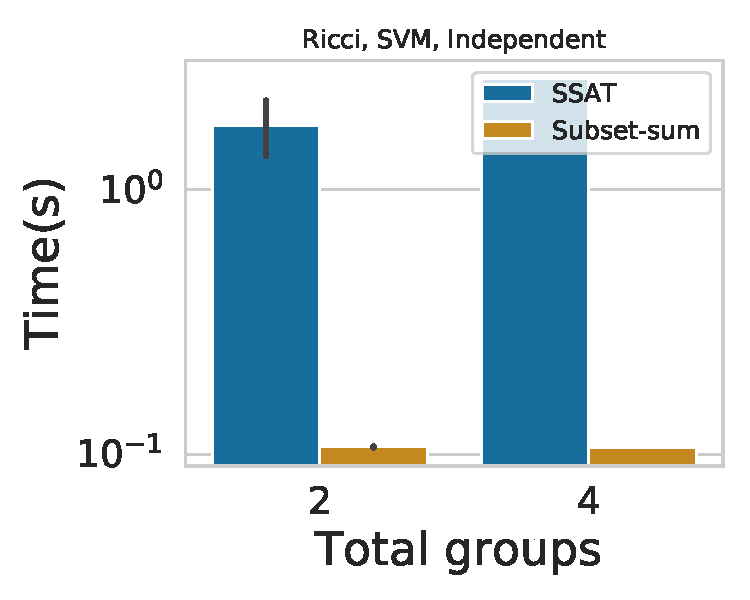
\includegraphics[scale=0.25]{figures/ssat_vs_subsetsum_Independent_Ricci_SVM}}
			\subfloat[]{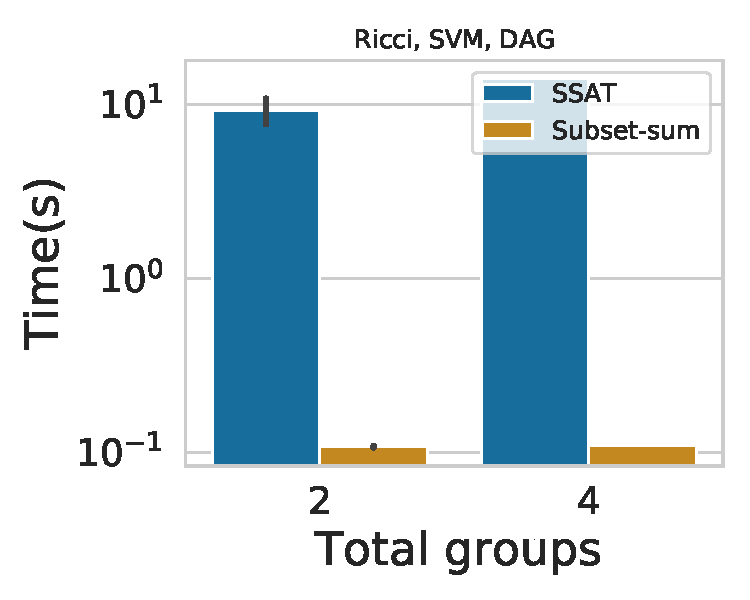
\includegraphics[scale=0.25]{figures/ssat_vs_subsetsum_DAG_Ricci_SVM}}
			\subfloat[]{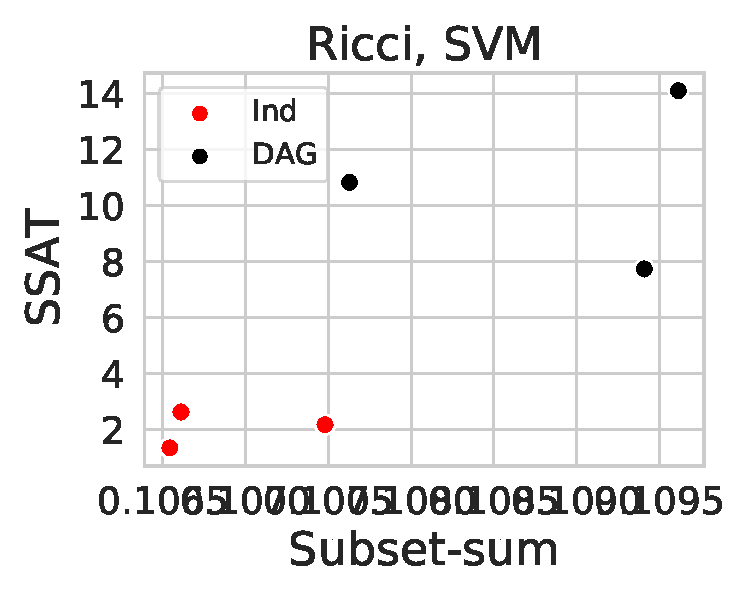
\includegraphics[scale=0.25]{figures/ssat_vs_subsetsum_time_scatter_plot_Ricci_SVM}}\\
			
			
			\subfloat[]{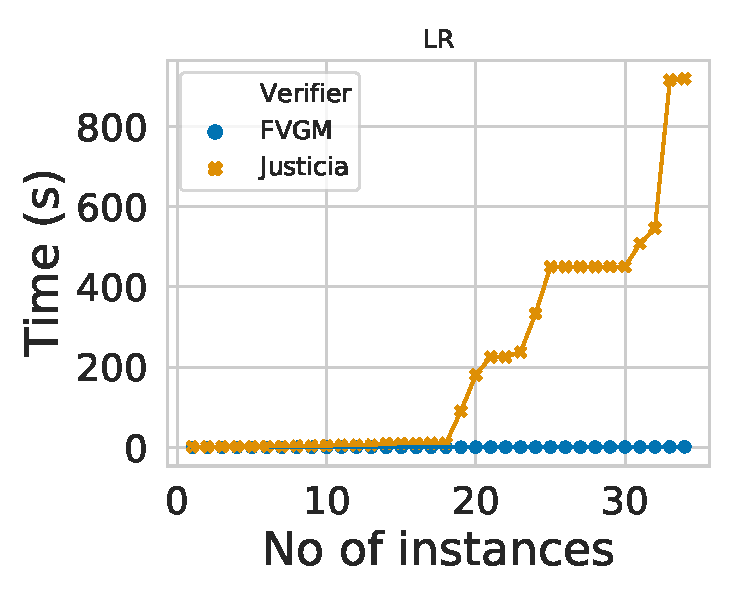
\includegraphics[scale=0.25]{figures/cactus_subsetsum_ssat_LR_time_.pdf}}
			\subfloat[]{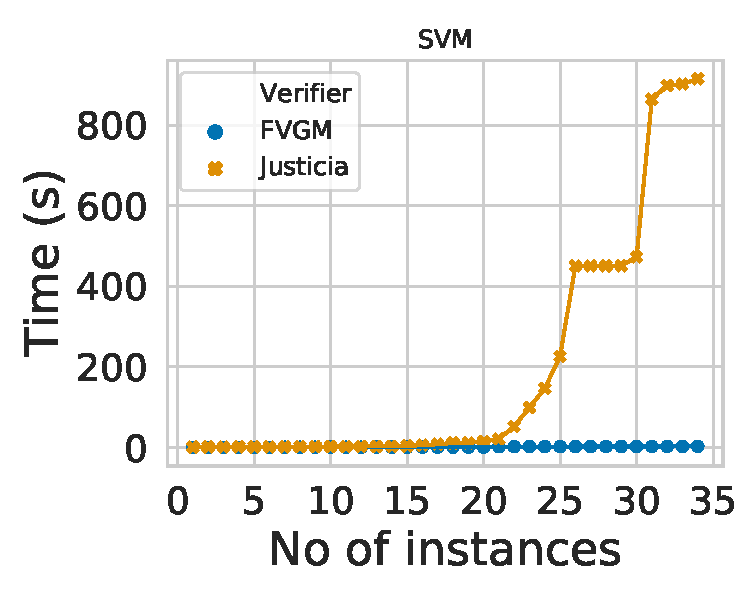
\includegraphics[scale=0.25]{figures/cactus_subsetsum_ssat_SVM_time_.pdf}}
			

		\end{center}
		
		\caption{Scalability between {\framework} and Justicia. \red{Each instance represents the runtime of verifying on a dataset and a set of sensitive attributes.}}
\end{figure}
	
	
	

	%
\begin{table*}       
    \centering
        \setlength{\tabcolsep}{.2em}
            \begin{tabular}{ll
            				ccc
            				ccc
            				ccc
            				ccc
            				ccc
            				ccc}
                \toprule
                \multirow{3}{*}{Encoding}& Dataset $ \rightarrow $   & 
                \multicolumn{8}{c}{Adult} &
%                \multicolumn{6}{c}{German} &
                \multicolumn{8}{c}{COMPAS} \\ 
                \cmidrule(lr){3-10}
                \cmidrule(lr){11-18}
                & Protected  $ \rightarrow $ & 
                \multicolumn{4}{c}{Race}   & \multicolumn{4}{c}{Sex}  &
%                \multicolumn{3}{c}{Age}   & \multicolumn{3}{c}{Sex}  &
                \multicolumn{4}{c}{Race}   & \multicolumn{4}{c}{Sex}
                \\ 
                \cmidrule(lr){3-6}
                \cmidrule(lr){7-10}
                \cmidrule(lr){11-14}
                \cmidrule(lr){15-18}

                 & Algorithm  $ \rightarrow $ &  
                orig. & RCO &
                orig. & CPP &
                orig. & RCO &
                orig. & CPP &
                orig. & RCO &
                orig. & CPP &
				orig. & RCO &
				orig. & CPP &
               \\
                \midrule
          
              
              
			Ind
			& DI&  $ 0.76 $ &  $ 0.67 $ &  $ 1.00 $ &  $ 0.71 $ &  $ 0.30 $ &  $ \mathbf{0.63} $ &  $ 1.00 $ &  $ 0.06 $ &  $ 0.96 $ &  $ 0.62 $ &  $ 1.00 $ &  $ \mathbf{1.00} $ &  $ 0.60 $ &  $ 0.55 $ &  $ 0.80 $ &  $ 0.75 $  \\
			& SP&  $ 0.15 $ &  $ 0.16 $ &  $ 0.00 $ &  $ 0.05 $ &  $ 0.53 $ &  $ \mathbf{0.21} $ &  $ 0.00 $ &  $ 0.13 $ &  $ 0.01 $ &  $ 0.14 $ &  $ 0.00 $ &  $ \mathbf{0.00} $ &  $ 0.13 $ &  $ \mathbf{0.13} $ &  $ 0.11 $ &  $ \mathbf{0.10} $  \\
			\midrule
			DAG
			& DI&  $ 0.73 $ &  $ 0.68 $ &  $ 1.00 $ &  $ 0.71 $ &  $ 0.33 $ &  $ \mathbf{0.68} $ &  $ 1.00 $ &  $ 0.05 $ &  $ 0.93 $ &  $ 0.62 $ &  $ 1.00 $ &  $ \mathbf{1.00} $ &  $ 0.62 $ &  $ 0.56 $ &  $ 0.80 $ &  $ 0.75 $  \\
			& SP&  $ 0.17 $ &  $ \mathbf{0.15} $ &  $ 0.00 $ &  $ 0.05 $ &  $ 0.51 $ &  $ \mathbf{0.17} $ &  $ 0.00 $ &  $ 0.15 $ &  $ 0.02 $ &  $ 0.14 $ &  $ 0.00 $ &  $ \mathbf{0.00} $ &  $ 0.13 $ &  $ \mathbf{0.13} $ &  $ 0.11 $ &  $ \mathbf{0.10} $  \\
			
			
               
            \bottomrule
    \end{tabular}
\caption{Logistic regression and two encodings: learn and learn-dependency. ``\textemdash'' refers to timeout of DAG learner (Notears). }
\end{table*}



\begin{table*}       
	\centering
	        \setlength{\tabcolsep}{.2em}
	\begin{tabular}{ll
			ccc
			ccc
			%            				ccc
			%            				ccc
			ccc
			ccc}
		\toprule
		\multirow{3}{*}{Classifier}& Dataset $ \rightarrow $   & 
		\multicolumn{6}{c}{Adult} &
		%                \multicolumn{6}{c}{German} &
		\multicolumn{6}{c}{COMPAS} \\ 
		\cmidrule(lr){3-8}
		\cmidrule(lr){9-14}
		%                \cmidrule(lr){15-20}
		& Protected  $ \rightarrow $ & 
		\multicolumn{3}{c}{Race}   & \multicolumn{3}{c}{Sex}  &
		%                \multicolumn{3}{c}{Age}   & \multicolumn{3}{c}{Sex}  &
		\multicolumn{3}{c}{Race}   & \multicolumn{3}{c}{Sex}
		\\ 
		\cmidrule(lr){3-5}
		\cmidrule(lr){6-8}
		\cmidrule(lr){9-11}
		\cmidrule(lr){12-14}
		%                \cmidrule(lr){15-17}
		%                \cmidrule(lr){18-20}
		
		& Algorithm  $ \rightarrow $ &  
		orig. & RW & OP & 
		orig. & RW & OP &
		%                orig. & RW & OP &
		%                orig. & RW & OP &
		orig. & RW & OP &
		orig. & RW & OP \\ 
		\midrule
		
		
		
		\multirow{3}{*}{\shortstack{Logistic \\ regression}}
		& Disparte impact&  $ 0.41 $ &  $ \mathbf{0.67} $ &  $ \mathbf{0.97} $ &  $ 0.04 $ &  $ \mathbf{1.00} $ &  $ \mathbf{0.76} $ &  $ 0.78 $ &  $ 0.49 $ &  $ 0.63 $ &  $ 0.64 $ &  $ 0.63 $ &  $ \mathbf{1.00} $  \\
		& Stat. parity&  $ 0.07 $ &  $ \mathbf{0.05} $ &  $ \mathbf{0.00} $ &  $ 0.16 $ &  $ \mathbf{0.00} $ &  $ \mathbf{0.02} $ &  $ 0.09 $ &  $ 0.31 $ &  $ 0.21 $ &  $ 0.16 $ &  $ 0.21 $ &  $ \mathbf{0.00} $  \\
		& Equalized odds&  $ 0.03 $ &  $ \mathbf{0.02} $ &  $ \mathbf{0.00} $ &  $ 0.08 $ &  $ \mathbf{0.00} $ &  $ \mathbf{0.06} $ &  $ 0.09 $ &  $ 0.31 $ &  $ 0.20 $ &  $ 0.17 $ &  $ 0.20 $ &  $ \mathbf{0.00} $  \\
		\midrule
		\multirow{3}{*}{\shortstack{Decision \\ tree}}
		& Disparte impact&  $ 0.65 $ &  $ \mathbf{1.00} $ &  $ \mathbf{0.80} $ &  $ 0.00 $ &  $ \mathbf{1.00} $ &  $ \mathbf{0.92} $ &  $ 0.96 $ &  $ \mathbf{0.97} $ &  $ \mathbf{1.00} $ &  $ 0.82 $ &  $ \mathbf{1.00} $ &  $ \mathbf{0.95} $  \\
		& Stat. parity&  $ 0.04 $ &  $ \mathbf{0.00} $ &  $ \mathbf{0.03} $ &  $ 0.17 $ &  $ \mathbf{0.00} $ &  $ \mathbf{0.01} $ &  $ 0.02 $ &  $ \mathbf{0.01} $ &  $ \mathbf{0.00} $ &  $ 0.07 $ &  $ \mathbf{0.00} $ &  $ \mathbf{0.02} $  \\
		& Equalized odds&  $ 0.12 $ &  $ \mathbf{-0.00} $ &  $ \mathbf{0.03} $ &  $ 0.45 $ &  $ \mathbf{0.00} $ &  $ \mathbf{0.06} $ &  $ 0.02 $ &  $ \mathbf{0.01} $ &  $ \mathbf{0.00} $ &  $ 0.07 $ &  $ \mathbf{0.00} $ &  $ \mathbf{0.06} $  \\
		
		
		
		
		
		
		
		
		\bottomrule
	\end{tabular}
	\caption{Verification of different fairness enhancing algorithms for multiple datasets and classifiers using {\framework}. Numbers in bold refer to fairness improvement  compared against the unprocessed (orig.) dataset. RW and OP refer to reweighing and optimized-preprocessing algorithm respectively. }
\end{table*}
	\begin{figure}
	\begin{center}
		\subfloat{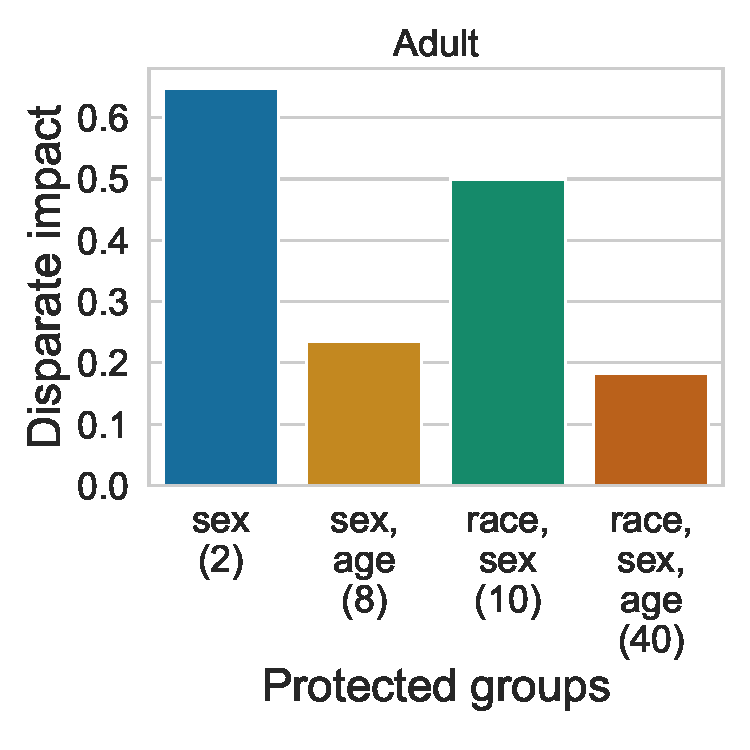
\includegraphics[scale=0.4]{figures/fairness/fvgm/sensitive_attribute__Disparate_impact_Adult_LR_Learn-efficient-dependency}}
		\subfloat{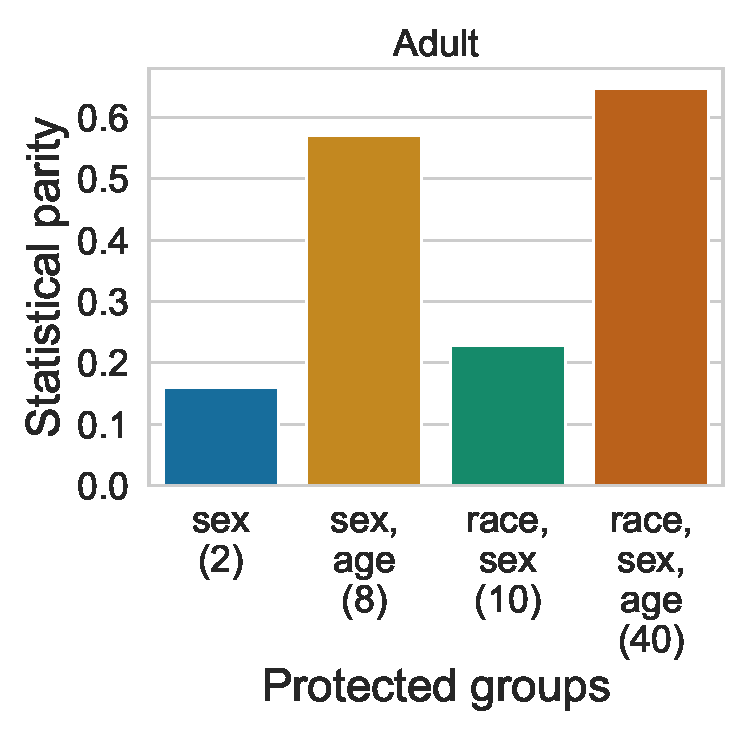
\includegraphics[scale=0.4]{figures/fairness/fvgm/sensitive_attribute__Statistical_parity_Adult_LR_Learn-efficient-dependency}}
		\vspace{-1em}
		
		\subfloat{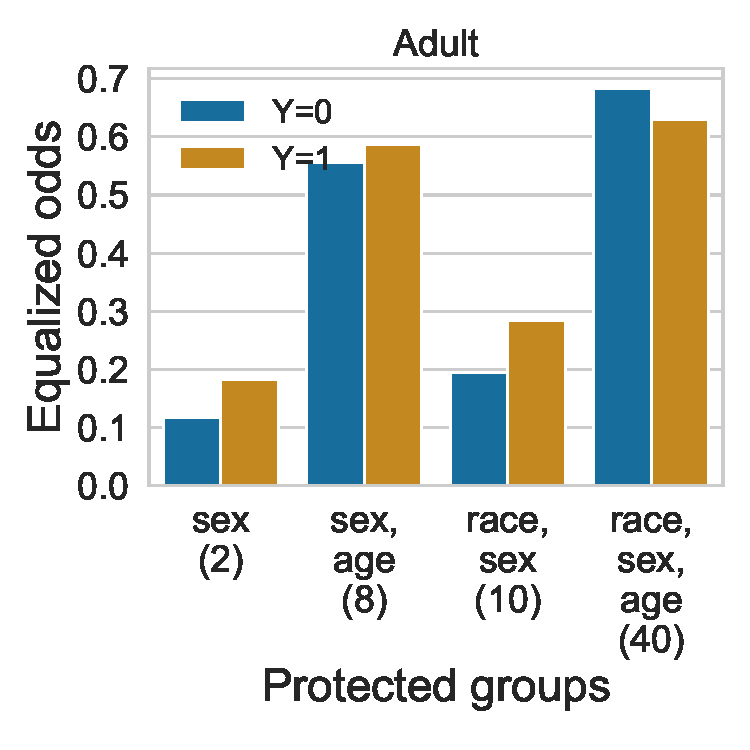
\includegraphics[scale=0.4]{figures/fairness/fvgm/sensitive_attribute_eqo_Adult_LR_Learn-efficient-dependency}}
		\subfloat{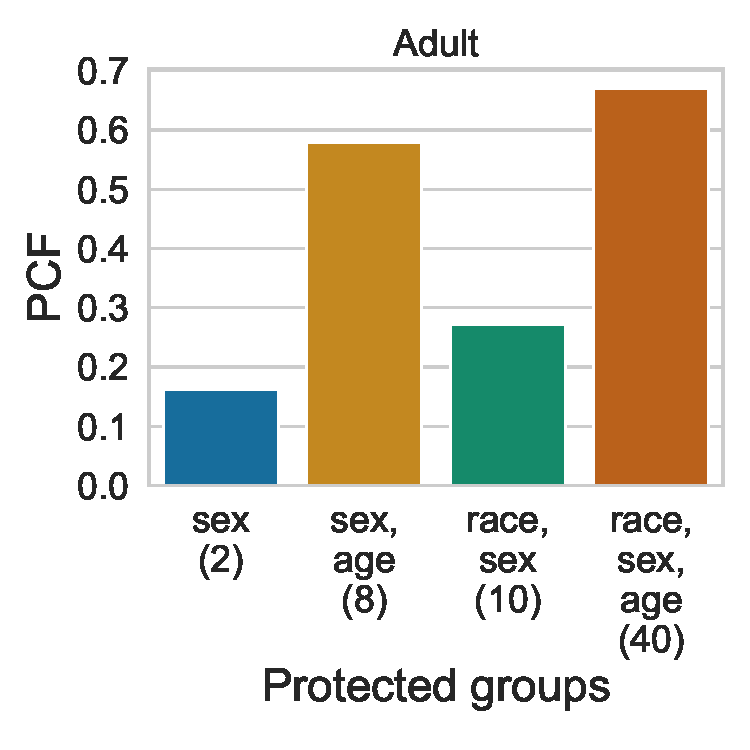
\includegraphics[scale=0.4]{figures/fairness/fvgm/sensitive_attribute__PCF_Adult_LR_Learn-efficient-dependency}}	
		\vspace{-1em}
		
		\subfloat{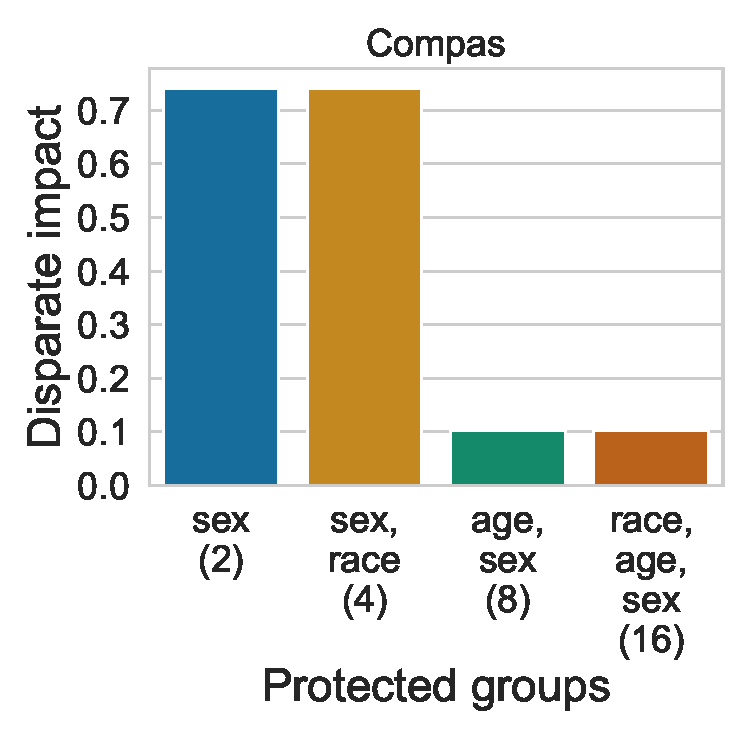
\includegraphics[scale=0.4]{figures/fairness/fvgm/sensitive_attribute__Disparate_impact_Compas_LR_Learn-efficient-dependency}}			
		\subfloat{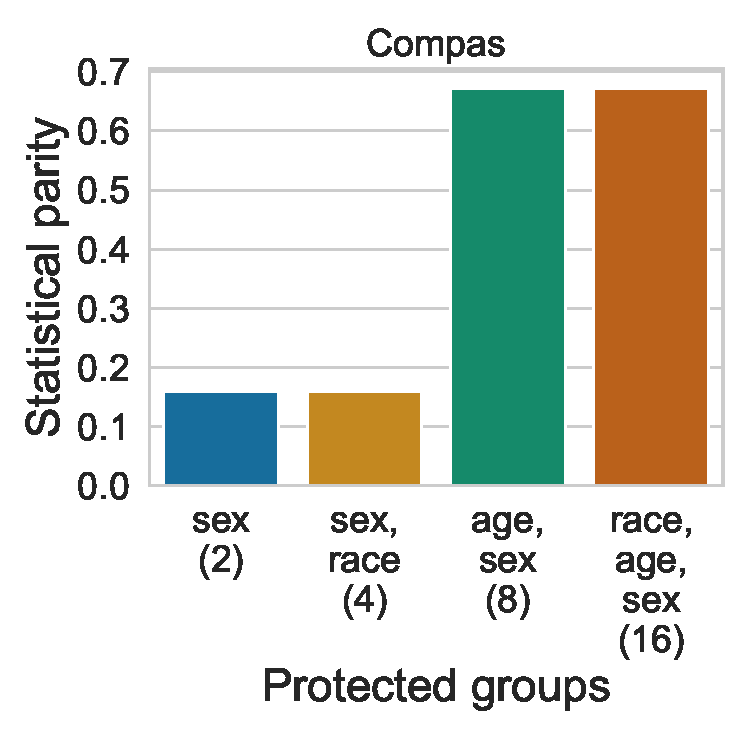
\includegraphics[scale=0.4]{figures/fairness/fvgm/sensitive_attribute__Statistical_parity_Compas_LR_Learn-efficient-dependency}}
		\vspace{-1em}
		
		\subfloat{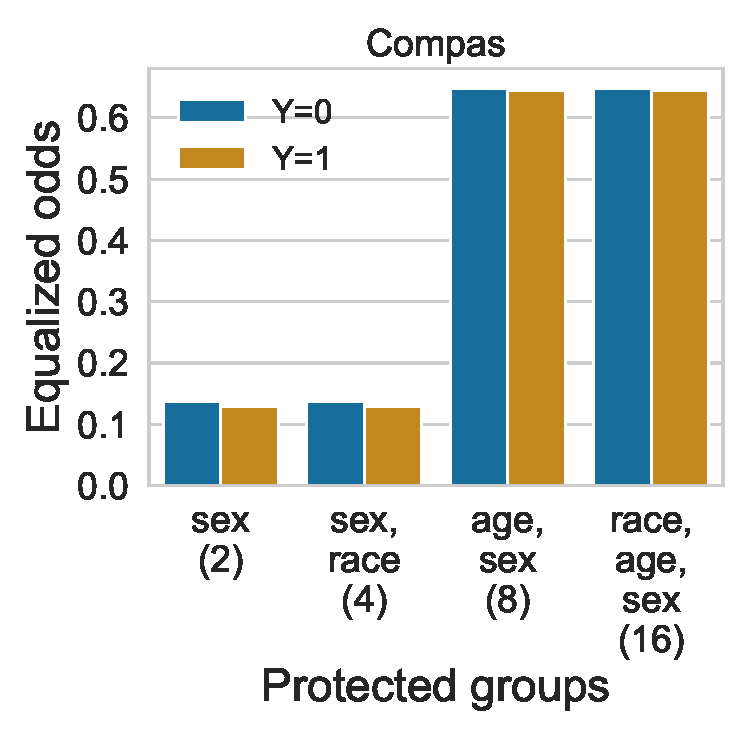
\includegraphics[scale=0.4]{figures/fairness/fvgm/sensitive_attribute_eqo_Compas_LR_Learn-efficient-dependency}}
		\subfloat{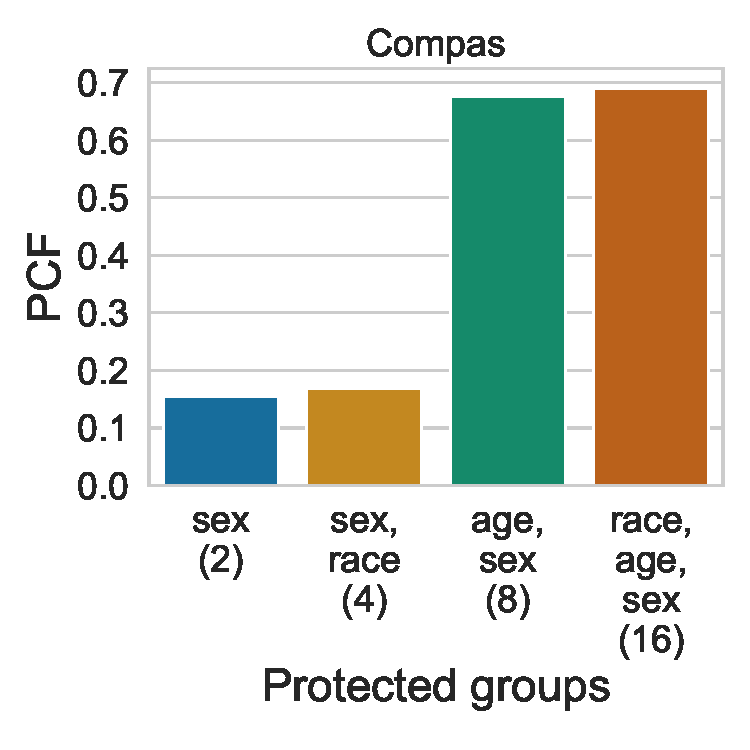
\includegraphics[scale=0.4]{figures/fairness/fvgm/sensitive_attribute__PCF_Compas_LR_Learn-efficient-dependency}}	
		
	\end{center}
		\caption{Verifying compound sensitive groups with respect to multiple fairness metrics. In each plot, the $ X $-axis shows sensitive features with the number of compound groups (within parenthesis) and $ Y $-axis shows computed group and causal fairness metrics. }
		\label{fairness_fvgm_fig:multiple_metrics}

\end{figure}
	
	
	
	
	\begin{figure}
		\begin{center}		
	
	\subfloat{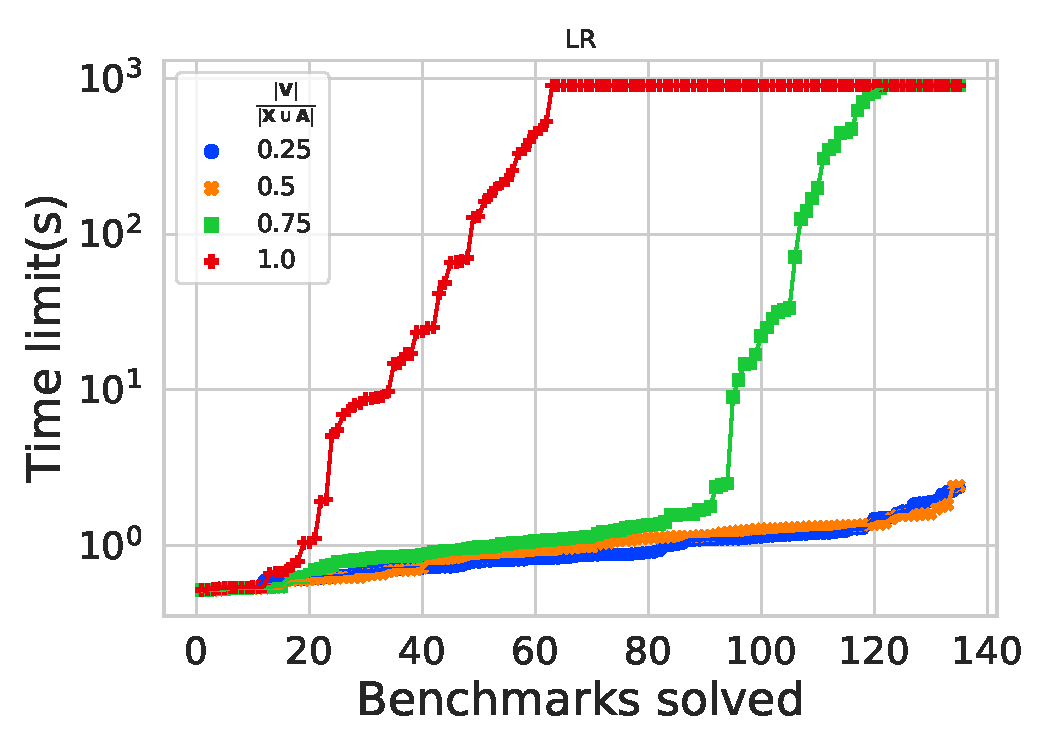
\includegraphics[scale=0.4]{figures/fairness/fvgm/cactus_dag_LR_time}}
	\subfloat{\includegraphics[scale=0.4]{figures/fairness/fvgm/cactus_dag_LR_time_notears}}
			
		\end{center}
		
		\caption[Ablation study: effect of Bayesian network on {\fvgm}]{Effect of number of variables in the learned Bayesian Network on computation time of {\fvgm}. In both plots, we vary $ \frac{|\mathbf{V}|}{|\nonsensitive \cup \sensitive|} $, that is the ratio between the number of variables in the Bayesian Network to the number of features. We observe that as this ratio increases to $ 1 $, both runtime of {\fvgm} (left plot) and network learning time (right plot) increase. } 
		\label{fairness_fvgm_fig:results_DAG_complexity}
\end{figure}
	
	
	

		
	\subsection{Verifying Fairness Algorithms on Multiple Fairness Metrics}
	
	We show extended results on verifying fairness attack in Figure~\ref{fairness_fvgm_fig:attack_extended} for two fairness metrics: disparate impact (DI) and statistical parity (SP). We observe that {\fvgm} can detect poisoning attack for both metrics. 	In Figure~\ref{fairness_fvgm_fig:multiple_metrics} we show verification results on compound sensitive groups with respect to multiple fairness metrics. In this figure, we observe that with an increase in the number of groups, fairness metrics worsens\textemdash disparate impact decreases and other three metrics increases.
		
	\subsection{Performance Analysis of Bayesian Network}
	In Figure~\ref{fairness_fvgm_fig:results_DAG_complexity}, we analyze the performance of encoding Bayesian Networks of differing complexity. We define the complexity of the network as  $ \frac{|V|}{|\nonsensitive \cup \sensitive|} $, which is the ratio between the number of features appearing in the network and total features. In this figure, as the ratio increases, both computation time of {\fvgm} and learning time of Bayesian Network increase. 
	
	
	\begin{comment}
	\begin{table}
	
	\centering
	\small
	\caption{Extended results for verification of different fairness enhancing algorithms using {\fvgm}. Numbers in bold refer to fairness improvement w.r.t. different fairness metrics. RW and OP refer to reweighing and optimized-preprocessing algorithms respectively.  }
	\label{fairness_fvgm_fig:extended_verifying_fairness_algorithms}
	\setlength{\tabcolsep}{.5em}
	
	\begin{tabular}{lllrrrrrrrrrrrrr}
		
		\toprule
		Dataset & Sensitive & Algo. & $ \Delta $DI &  $ \Delta $PCF & $ \Delta $SP & $ \Delta$ EO\\
		\midrule
		
		
		\multirow{4}{*}{Adult}&\multirow{2}{*}{race}&RW&$ \textbf{0.53} $&$ \textbf{-0.06} $&$ \textbf{-0.06} $&$ \textbf{-0.02} $\\
		&&OP&$ \textbf{0.57} $&$ \textbf{-0.07} $&$ \textbf{-0.07} $&$ \textbf{-0.02} $\\
		\cmidrule{2-7}
		&\multirow{2}{*}{sex}&RW&$ \textbf{0.96} $&$ \textbf{-0.16} $&$ \textbf{-0.15} $&$ \textbf{-0.08} $\\
		&&OP&$ \textbf{0.43} $&$ \textbf{-0.08} $&$ \textbf{-0.08} $&$ 0.03 $\\
		
		\midrule
		\multirow{4}{*}{COMPAS}&\multirow{2}{*}{race}&RW&$ \textbf{0.13} $&$ \textbf{-0.07} $&$ \textbf{-0.07} $&$ \textbf{-0.06} $\\
		&&OP&$ \textbf{0.15} $&$ \textbf{-0.08} $&$ \textbf{-0.08} $&$ \textbf{-0.05} $\\
		\cmidrule{2-7}
		&\multirow{2}{*}{sex}&RW&$ \textbf{0.1} $&$ \textbf{-0.04} $&$ \textbf{-0.04} $&$ 0.04 $\\
		&&OP&$ \textbf{0.09} $&$ \textbf{-0.04} $&$ \textbf{-0.04} $&$ \textbf{-0.03} $\\
		
		\midrule
		\multirow{4}{*}{German}&\multirow{2}{*}{age}&RW&$ \textbf{0.52} $&$ \textbf{-0.53} $&$ \textbf{-0.52} $&$ \textbf{-0.47} $\\
		&&OP&$ \textbf{0.53} $&$ \textbf{-0.53} $&$ \textbf{-0.53} $&$ \textbf{-0.51} $\\
		\cmidrule{2-7}
		&\multirow{2}{*}{sex}&RW&$ -0.06 $&$ 0.06 $&$ 0.06 $&$ 0.02 $\\
		&&OP&$ -0.12 $&$ 0.12 $&$ 0.12 $&$ 0.07 $\\
		
		
		\bottomrule
	\end{tabular}
\end{table}
	
	\end{comment}

	
\iffalse
\begin{table}[h!]
		\centering
		\caption{Extended results for runtime of different verifiers in seconds.  `\textemdash'~ refers to timeout ($ 900 $ seconds). Bold number refers to best scalability results. We additionally show results for decision tree classifiers (DT). {\fvgm} takes comparatively more time for decision tree classifiers because of encoding feature-correlations represented as a Bayesian network.}
			\label{fairness_fvgm_tab:scalability_extended}	
		\begin{tabular}{llrrrrrrrrrrrrrr}
			
			\toprule
			Dataset & Classifier & FairSquare & VeriFair & Justicia & {\fvgm} \\
			\midrule
			
			\multirow{3}{*}{Ricci} & LR & \textemdash &  $ 2.0 $  &  $ 2.2 $  &  $ \textbf{0.1} $  \\ 
			& SVM & \textemdash &  $ 1.8 $  &  $ 2.2 $  &  $ \textbf{0.1} $  \\ 
			& DT &  $ 4.6 $  &  $ 1.9 $  &  $ \textbf{0.1} $  &  $ \textbf{0.1} $  \\ 
			
			
			\midrule
			\multirow{3}{*}{Titanic} & LR & \textemdash &  $ 0.5 $  &  $ 0.3 $  &  $ \textbf{0.1} $  \\ 
			& SVM & \textemdash &  $ 0.4 $  &  $ 0.2 $  &  $ \textbf{0.1} $  \\ 
			& DT &  $ 432.9 $  &  $ 17.2 $  &  $ \textbf{0.3} $  &  $ 1.6 $  \\ 
			
			
			\midrule
			\multirow{3}{*}{Compas} & LR & \textemdash &  $ 12.2 $  & \textemdash &  $ \textbf{0.4} $  \\ 
			& SVM & \textemdash &  $ 11.6 $  & \textemdash &  $ \textbf{0.5} $  \\ 
			& DT & \textemdash &  $ 377.1 $  &  $ \textbf{0.3} $  &  $ 121.7 $  \\ 
			
			
			\midrule
			\multirow{3}{*}{Adult} & LR & \textemdash &  $ 7.3 $  & \textemdash &  $ \textbf{0.9} $  \\ 
			& SVM & \textemdash &  $ 21.7 $  &  $ \textbf{1.7} $  &  $ 1.8 $  \\ 
			& DT & \textemdash &  $ 57.9 $  &  $ 0.4 $  &  $ \textbf{0.3} $  \\ 
			
			
			\midrule
			\multirow{3}{*}{German} & LR & \textemdash &  $ 19.2 $  & \textemdash &  $ \textbf{1.4} $  \\ 
			& SVM & \textemdash &  $ 28.8 $  & \textemdash &  $ \textbf{1.4} $  \\ 
			& DT & \textemdash &  $ 78.5 $  &  $ \textbf{0.2} $  &  $ 2.3 $  \\ 
			
			
			\bottomrule
			
			
		\end{tabular}
		
	\end{table}	
\fi		

%\newpage
%\clearpage
\section{Fairness Influence Functions (FIF)}
Now, we present an elaborate discussion on computing fairness influence functions.
A Fairness Influence Function, denoted as $ \mathsf{FIF}(\cdot) $, is computed with respect to a \textit{quantity of interest}, for example, the  PPV of the classifier or different fairness metrics such as DI and SP. Let $ \mathbf{S}  \subseteq \nonsensitive $ be a set of non-sensitive features, for which we are interested in computing their influence. A general approach to compute $ \mathsf{FIF}(\mathbf{S}) $ is to replace each feature in $ \mathbf{S} $ with random values and report differences in the quantity of interest~\cite{datta2016algorithmic}. Let $ \mathcal{X}'_i $ denote the modified marginal distribution where we replace feature $ X_i \in \mathbf{S} $ with random values. For example, $ \mathcal{X}'_i $ can be viewed as an uniform distribution within the support of $ X_i $. We then define the modified product distribution, denoted as $ \mathcal{D}_{-\mathbf{S}} $ by combining all marginal distributions, where each feature in $ \mathbf{S} $ has a modified distribution. 
\[
\mathcal{D}_{-\mathbf{S}} = \prod_{i | X_i \in \mathbf{S}} \mathcal{X}'_i \prod_{i | X_i \in X \setminus \mathbf{S}} \mathcal{X}_i \prod_{j=1}^{n} \mathcal{A}_j 
\]
We first give a general definition of influence function of $ \mathbf{S} $ on a quantity, say $ Q $, in the following. 
\[
\mathsf{FIF}(\mathbf{S}) \triangleq Q(\mathcal{D}) - Q(\mathcal{D}_{-\mathbf{S}})
\]
Intuitively, influence of $ \mathbf{S} $ is the difference in a quantity computed for the original distribution $ \mathcal{D} $ and the modified distribution $ \mathcal{D}_{-\mathbf{S}} $. In the following, we define influence function in terms of PPV of the classifier. 
\[
\mathsf{FIF}_{\mathsf{PPV}}(\mathbf{S}) \triangleq \Pr[\hat{Y} = 1 | \mathcal{D}] - \Pr[\hat{Y} = 1 | \mathcal{D}_{-\mathbf{S}}]
\]
Influence function also generalizes to PPV specific to compound sensitive groups. For a sensitive group $ \mathbf{a} \in \sensitive $, we define group-specific influence as follows. 

\[
\mathsf{FIF}_{\mathsf{PPV},\; \mathbf{a}}(\mathbf{S}) \triangleq \Pr[\hat{Y} = 1 | \sensitive = \mathbf{a}, \mathcal{D}] - \Pr[\hat{Y} = 1 | \sensitive = \mathbf{a},  \mathcal{D}_{-\mathbf{S}}]
\]

\paragraph{Experimental Analysis.} We empirically instantiate computation of FIF and its consequences for a logistic regression classifier on COMPAS and Adult datasets.

For both the datasets, we consider biological `sex' as the sensitive features.
In both cases, we denote the sensitive groups `male' and `female' as `sex=0' and `sex=1', respectively. 
FIFs computed for these sensitive groups show influence of different features and their relevant disparities. We illustrate the results in Figure~\ref{fairness_fvgm_fig:fif}.

Figure~\ref{fairness_fvgm_fig:fif_a} illustrates that the PPV value for the `male' population in the dataset is $0.61$. If we now replace the feature `age' with uniformly random values, the PPV for the same group becomes $0.46$, Thus, the FIF of the feature `age' for `male' group is $0.15$.
Similarly, all the red bars in Figures~\ref{fairness_fvgm_fig:fif_a}-\ref{fairness_fvgm_fig:fif_b}, ~\ref{fairness_fvgm_fig:fif_c}-\ref{fairness_fvgm_fig:fif_d} indicate a positive influence of that feature and the green bars indicate a negative influence of the feature on the individual getting classified to $\hat{Y}=1$.

In Figures~\ref{fairness_fvgm_fig:fif_c} and~\ref{fairness_fvgm_fig:fif_f}, we illustrate the influence of different features on the disparate impact between the two groups `male' and `female'. 
The green bar indicates that removing a feature causes an increase in DI, i.e. fairness in classification, and the red bar indicates the opposite. Alternatively, we can conclude that bigger is the green bar for a feature, higher is the bias-inducing effect of it.

Thus, from Figure~\ref{fairness_fvgm_fig:fif_c}, we conclude that `age' is the most bias-inducing feature among the two groups `male' and `female'.
From Fig~\ref{fairness_fvgm_fig:fif_a} and~\ref{fairness_fvgm_fig:fif_b}, we observe that `age' is a decisive feature for `male' while it is comparatively insignificant for `female'.

In case of Adult dataset, the PPV for `male' and `female' groups are 0.45 and 0.3 respectively. Among all the features, we observe that `race' has a positive impact on the classification for both the groups. This means removing the `race' information decreases the chance of getting classified to higher economic group. On the other hand, `capital-gain' has the highest influence on the classification for both groups. It is also the most biased-inducing feature as it varies most disparately among the two groups as the `capital-gain' differs significantly between two groups. 
\begin{figure}
	\begin{center}
	
		\subfloat[COMPAS]{\includegraphics[scale=0.35]{figures/fairness/fvgm/dependency_exp_Learn-dependency_compas_lr_sex_0}\label{fairness_fvgm_fig:fif_a}}
		\subfloat[COMPAS]{\includegraphics[scale=0.35]{figures/fairness/fvgm/dependency_exp_Learn-dependency_compas_lr_sex_1}\label{fairness_fvgm_fig:fif_b}}\\
		\subfloat[Adult]{\includegraphics[scale=0.35]{figures/fairness/fvgm/dependency_exp_Learn-dependency_adult_lr_sex_0}\label{fairness_fvgm_fig:fif_d}}
		\subfloat[Adult]{\includegraphics[scale=0.35]{figures/fairness/fvgm/dependency_exp_Learn-dependency_adult_lr_sex_1}\label{fairness_fvgm_fig:fif_e}}\\
		\subfloat[COMPAS]{\includegraphics[scale=0.35]{figures/fairness/fvgm/dependency_exp_Learn-dependency_compas_lr_sex_DI}\label{fairness_fvgm_fig:fif_c}}
		\subfloat[Adult]{\includegraphics[scale=0.35]{figures/fairness/fvgm/dependency_exp_Learn-dependency_adult_lr_sex_DI}\label{fairness_fvgm_fig:fif_f}}\\
		
	
		
	\end{center}
	\caption[FIF illustration using {\fvgm}]{Extended results on computing feature influence functions (FIF) for COMPAS  and Adult dataset.}\label{fairness_fvgm_fig:fif}
\end{figure}





\iffalse
\clearpage
\paragraph{Limitations of existing SSAT solvers.}
Since there is no state of the art SSAT solver that can handle universal quantification, we cannot consider conditional probabilities of universal variables while encoding the Bayesian network. In {\fvgm}, universal quantification appears while learning the least favored group in the learning encoding. When we do not consider conditional probabilities on universal variables, earlier approach could solve this using an existential SSAT solver by first negating the CNF and then subtracting computed probability from $ 1 $ as a solution to the original universal SSAT problem. This approach does not work when conditional probabilities are involved. 

For example, consider a clause $ a \vee\mathbf{B}\vee c $ defined on three Boolean variables where $ a $ is existential and $ b,c $ are random. Without considering conditional probabilities on $ a $, it is assigned true trivially. However, with conditional probabilities $ a $ can be false depending on the probability. Similar argument holds when $ a $ is universal. Hence, when conditional probabilities are considered for universal variables, a dedicated SSAT solver is also required to solve them. 
\fi





%\noindent\makebox[\linewidth]{\rule{\textwidth}{0.4pt}}	




\appendix

\chapter{Feature Correlations in SSAT-based Fairness Verifier: {\justicia}}
\label{chapter:CNF_feature_correlation}
In Chapter~\ref{chapter:justicia}, {\justicia} verifies the fairness of CNF classifiers without considering correlation among features. In this chapter, we address fairness verification of CNF classifiers with correlated features. In particular, we present the encoding of conditional probabilities from a Bayesian network into the SSAT formulation in {\justicia}. 







\subsection*{Methodology}
For CNF classifiers, SSAT is a natural choice as it computes the probability of satisfaction of a CNF formula  given quantified Boolean variables, where quantifiers distinguish between (random) non-sensitive variables and (existential or universal) sensitive variables. Let $ \phi_{\widehat{Y}} $ be a CNF classifier such that a satisfying assignment of $ \phi_{\widehat{Y}} $ denotes the positive prediction of the classifier $ \widehat{Y} = 1 $. We consider another CNF formula $ \phi_\BN $ to encode the conditional dependencies among variables in the Bayesian Network $ \BN $, which is given as the input distribution. $ \phi_\BN $ contains auxiliary variables to encode the conditional dependencies, which we discuss shortly. The outline of our methodology is to construct a conjoined CNF formula $ \phi_{\widehat{Y}} \wedge \phi_\BN $, assign appropriate quantifiers to the variables, and solve an SSAT problem on quantified formula $ \phi_{\widehat{Y}} \wedge \phi_\BN $ to answer queries such as $ \max_{\mathbf{a}} \Pr[\widehat{Y} = 1 | \sensitive = \mathbf{a}] $ and $ \min_{\mathbf{a}} \Pr[\widehat{Y} = 1 | \sensitive = \mathbf{a}] $\textemdash the maximum and minimum conditional positive prediction of the classifiers with correlated features, respectively.




\paragraph{Encoding a Bayesian Network as a CNF Formula.}\label{sec:BN_to_CNF}
Our goal is to encode the Bayesian network $ \BN = (\graph, \factors) $ into a CNF formula $ \phi_\BN $ such that \textit{the weighted model count} of $ \phi_\BN $ exactly computes the joint probability distribution in $ \BN $~\cite{chavira2008probabilistic}.  In this context, an SSAT formula trivially does not allow conditional probabilities of randomized quantified variables. Hence, $ \phi_\BN $ contains additional \textit{auxiliary variables} to capture the conditional probabilities, as discussed next.


Let  $ G = (\mathbf{V}, \mathbf{E}) $ where $  $  $ \mathbf{V} \subseteq \nonsensitive \cup \sensitive $, $ \mathbf{E} \subseteq \mathbf{V} \times \mathbf{V} $, and each variable $ V_i \in \mathbf{V} $ is Boolean. For each network variable $ V_i \in \mathbf{V} $, we define a Boolean \textit{indicator}  variable $ \lambda_{V_i} $ such that $ \Pr[\lambda_{V_i}] \triangleq \Pr[V_i] $. We add following constraint in $ \phi_\BN $ to establish the relation between $ \lambda_{V_i} $ and $ V_i $. 
\begin{align}
\lambda_{V_i} \leftrightarrow V_i,
\label{eq:indicator_constraint}
\end{align}
Intuitively, both $ \lambda_{V_i} $ and $ V_i $ are either true or false. This constraint can be trivially translated to clauses in CNF using the equivalence rule $ A \leftrightarrow B \equiv (\neg A \vee B)  \wedge (A \vee \neg B) $ for Boolean variables $ A, B$.

We now present the encoding of conditional probabilities induced by parameters in the network $ \theta $. Let $ V_i \in  \mathbf{V}  $  be a vertex in $ G $ where $ \parent(V_i) \ne \emptyset $ be $ V_i $'s parents and $ |\parent(V_i)| = k $. Additionally, let $ v $ and $ \mathbf{u} \triangleq [u_1,.., u_k] $ be an assignment of  $ V_i $ and $ \parent(V_i)  $, respectively.  To encode $ \Pr[V_i = v| \parent(V_i) = \mathbf{u}]$, we introduce auxiliary variable $ \lambda_{v,\mathbf{u}} $ and add following constraints in $ \phi_{\BN} $.
\begin{align}
\lambda_{v,\mathbf{u}}  \wedge \bigwedge_{j=1}^{k} \lambda_{u_j} \rightarrow \lambda_v
\label{eq:factor_pos}
\end{align}
\begin{align}
\neg \lambda_{v,\mathbf{u}}  \wedge \bigwedge_{j=1}^{k} \lambda_{u_j} \rightarrow \neg \lambda_v
\label{eq:factor_neg}
\end{align}

where $ \lambda_v \equiv \lambda_{V_i} $. Moreover, $ \lambda_{u_j} $ is the indicator variable corresponding to the $ j^\text{th} $ parent in $ \parent(V_i) $. In the above two constraints,	for a fixed assignment $ \mathbf{u} $ of parents $ \parent(V_i) $, both $ \lambda_v $ and $ \lambda_{v,\mathbf{u}} $ are either true or false.  Hence, these two constraints encode the conditional probability of $ V_i = v $ given $ \parent(V_i) = \mathbf{u} $ using $ \Pr[\lambda_{v,\mathbf{u}}] = \Pr[V_i = v| \parent(V_i) = \mathbf{u}]$. Both constraints can be translated to CNF clauses trivially. For example, Eq.~\ref{eq:factor_pos} is translated as $ \neg \lambda_{v,\mathbf{u}}  \vee \bigvee_{j=1}^{k} \neg \lambda_{u_j} \vee \lambda_v $. We next analyze the complexity of $ \phi_\BN $ in terms of the number of variables and clauses.

\begin{lemma}
	For a Bayesian network $ \BN = (\graph, \factors) $ defined over $ n $ Boolean variables and $ \bncomplexity(\graph) $ network complexity, the encoded CNF formula $ \phi_\BN $ has $ n + \bncomplexity(\graph) $  variables and $ 2(n + \bncomplexity(\graph)) $ clauses. 
\end{lemma}
\begin{proof}
	Since the DAG in the Bayesian network has $ n $ vertices, we consider $ n $ indicator variables. Moreover, for encoding conditional probabilities, we consider $ \bncomplexity(\graph) $ auxiliary variables where $ \bncomplexity(\graph) $ denotes the the number of independent parameters in the network (ref. Chapter~\ref{chapter_fairness_preliminaries_BN}). Hence, total variables in $ \phi_\BN $ is $ n + \bncomplexity(\graph)  $.
	
	According to Eq.~\eqref{eq:indicator_constraint},~\eqref{eq:factor_pos},~\eqref{eq:factor_neg}, there are $2( n + \bncomplexity(\graph)) $ clauses in $ \phi_\BN $.
	
	
\end{proof}



\paragraph{Quantifiers in $ \phi_{\widehat{Y}} \wedge \phi_\BN $.}
We now discuss the quantifiers in $ \phi_{\widehat{Y}} \wedge \phi_\BN $, the SSAT solution of which  constitutes the maximum (minimum) probability of positive prediction of a CNF classifier. $ \phi_{\widehat{Y}} \wedge \phi_\BN $ contains four  categories of variables : (i) sensitive variables $ \sensitive $, (ii) non-sensitive variables $ \nonsensitive $, (iii) indicator variables $  \lambda_{V_i} $, and (iv) auxiliary variables $ \lambda_{v,\mathbf{u}} $. Among them, (iii) and (iv) are associated with $ \phi_\BN $ and the rest for $ \phi_{\widehat{Y}} $. For computing the maximum probability of positive prediction of the classifier, we construct  an exists-random-exists (ERE) SSAT formula with following quantifiers: we set sensitive features $ \sensitive $ with existential quantifiers in the beginning of the prefix of the SSAT formula followed by $  \lambda_{V_i}, \lambda_{v,\mathbf{u}} $, and $ X_j \in \nonsensitive \setminus \mathbf{V} $ with randomized quantifiers. The remaining variables  $ X_i \in \mathbf{V} $ are existentially quantified as their assignment is fixed by indicator variables $ \lambda_{V_i} $. In contrast, for computing the minimum probability of positive prediction of the classifier, we consider an universal-random-exists (URE) SSAT formula  where we set sensitive features $ \sensitive $ as universal quantifiers with all other quantifiers remaining same.






